% appendices/license_plate_detection_results.tex

\section{License Plate Detection Results}
\label{app:license_plate_results}

This appendix documents the evaluation results for the custom-trained license
plate detection model. The model was trained using the same YOLOX-based
training pipeline as the barcode detection model described in
Section~\ref{sec:....}. Therefore, this appendix only
presents the supporting results used to evaluate the license plate detector.


\subsection{Training Setup}

\begin{table}[H]
\centering
\begin{tabular}{lccc}
\toprule
Total Images & Training & Validation & Testing \\
\midrule
36959 & 31413 & 3697 & 1849 \\
\bottomrule
\end{tabular}
\caption{Image split used for the license plate detection experiments.}
\label{tab:license_plate_training_split}
\end{table}

The dataset was divided into approximately 85\% training, 10\% validation, and
5\% testing. After excluding three label files, the dataset consisted of 36,959 images. This split was chosen to provide a large number of training
samples while still reserving separate validation and test sets for monitoring
training performance and evaluating the final model on unseen data. Both models
used the same training, validation, and test split.


\begin{table}[H]
\centering

\begin{minipage}[t]{0.43\textwidth}
\centering
\caption{Training Configuration for Model V0}
\label{tab:lp_training_config_v0}
\scriptsize
\renewcommand{\arraystretch}{1.05}
\begin{tabular}{>{\raggedright\arraybackslash}p{0.52\linewidth}
                >{\raggedright\arraybackslash}p{0.38\linewidth}}
\toprule
\textbf{Parameter} & \textbf{Value} \\
\midrule
Architecture & YOLOX-S \\
Input Resolution & $640 \times 640$ \\
Batch Size & 16 \\
Max Epochs & 200 \\
No-Aug. Epochs & 15 \\
\midrule
\textit{Optimization} & \\
Base Learning Rate & 0.01 / 64 \\
Warmup Epochs & 5 \\
Min LR Ratio & 0.05 \\
Optimizer & SGD \\
\midrule
\textit{Augmentation (Offline)} & \\
Mosaic Images & 0.8 (0.3--1.8) \\
Color / Flip & 0.5 / 0.5 \\
Rotation / Shift / Shear & 5.0 / 0.05 / 1.0 \\
Random Image Size & (10, 20) \\
\midrule
\textit{Hardware} & \\
GPU Model & RTX 4080 \\
\bottomrule
\end{tabular}
\end{minipage}
\hfill
\begin{minipage}[t]{0.43\textwidth}
\centering
\caption{Training Configuration for Model V1}
\label{tab:lp_training_config_v1}
\scriptsize
\renewcommand{\arraystretch}{1.05}
\begin{tabular}{>{\raggedright\arraybackslash}p{0.52\linewidth}
                >{\raggedright\arraybackslash}p{0.38\linewidth}}
\toprule
\textbf{Parameter} & \textbf{Value} \\
\midrule
Architecture & YOLOX-S \\
Input Resolution & $960 \times 960$ \\
Batch Size & 8 \\
Max Epochs & 200 \\
No-Aug. Epochs & 15 \\
\midrule
\textit{Optimization} & \\
Base Learning Rate & 0.01 / 64 \\
Warmup Epochs & 5 \\
Min LR Ratio & 0.05 \\
Optimizer & SGD \\
\midrule
\textit{Augmentation (Offline)} & \\
Mosaic Images & 0.8 (0.5--1.5) \\
Color / Flip & 0.5 / 0.5 \\
Rotation / Shift / Shear & 5.0 / 0.05 / 1.0 \\
Random Image Size & (14, 24) \\
\midrule
\textit{Hardware} & \\
GPU Model & RTX 4080 \\
\bottomrule
\end{tabular}
\end{minipage}

\end{table}

Tables~\ref{tab:lp_training_config_v0} and~\ref{tab:lp_training_config_v1}
summarize the training configurations for the two license plate detection
models. The main difference was the increased input resolution in v1, which
required a smaller batch size.



\subsection{Training Curves}


\begin{figure}[H]
\centering

\begin{subfigure}{0.50\textwidth}
\centering
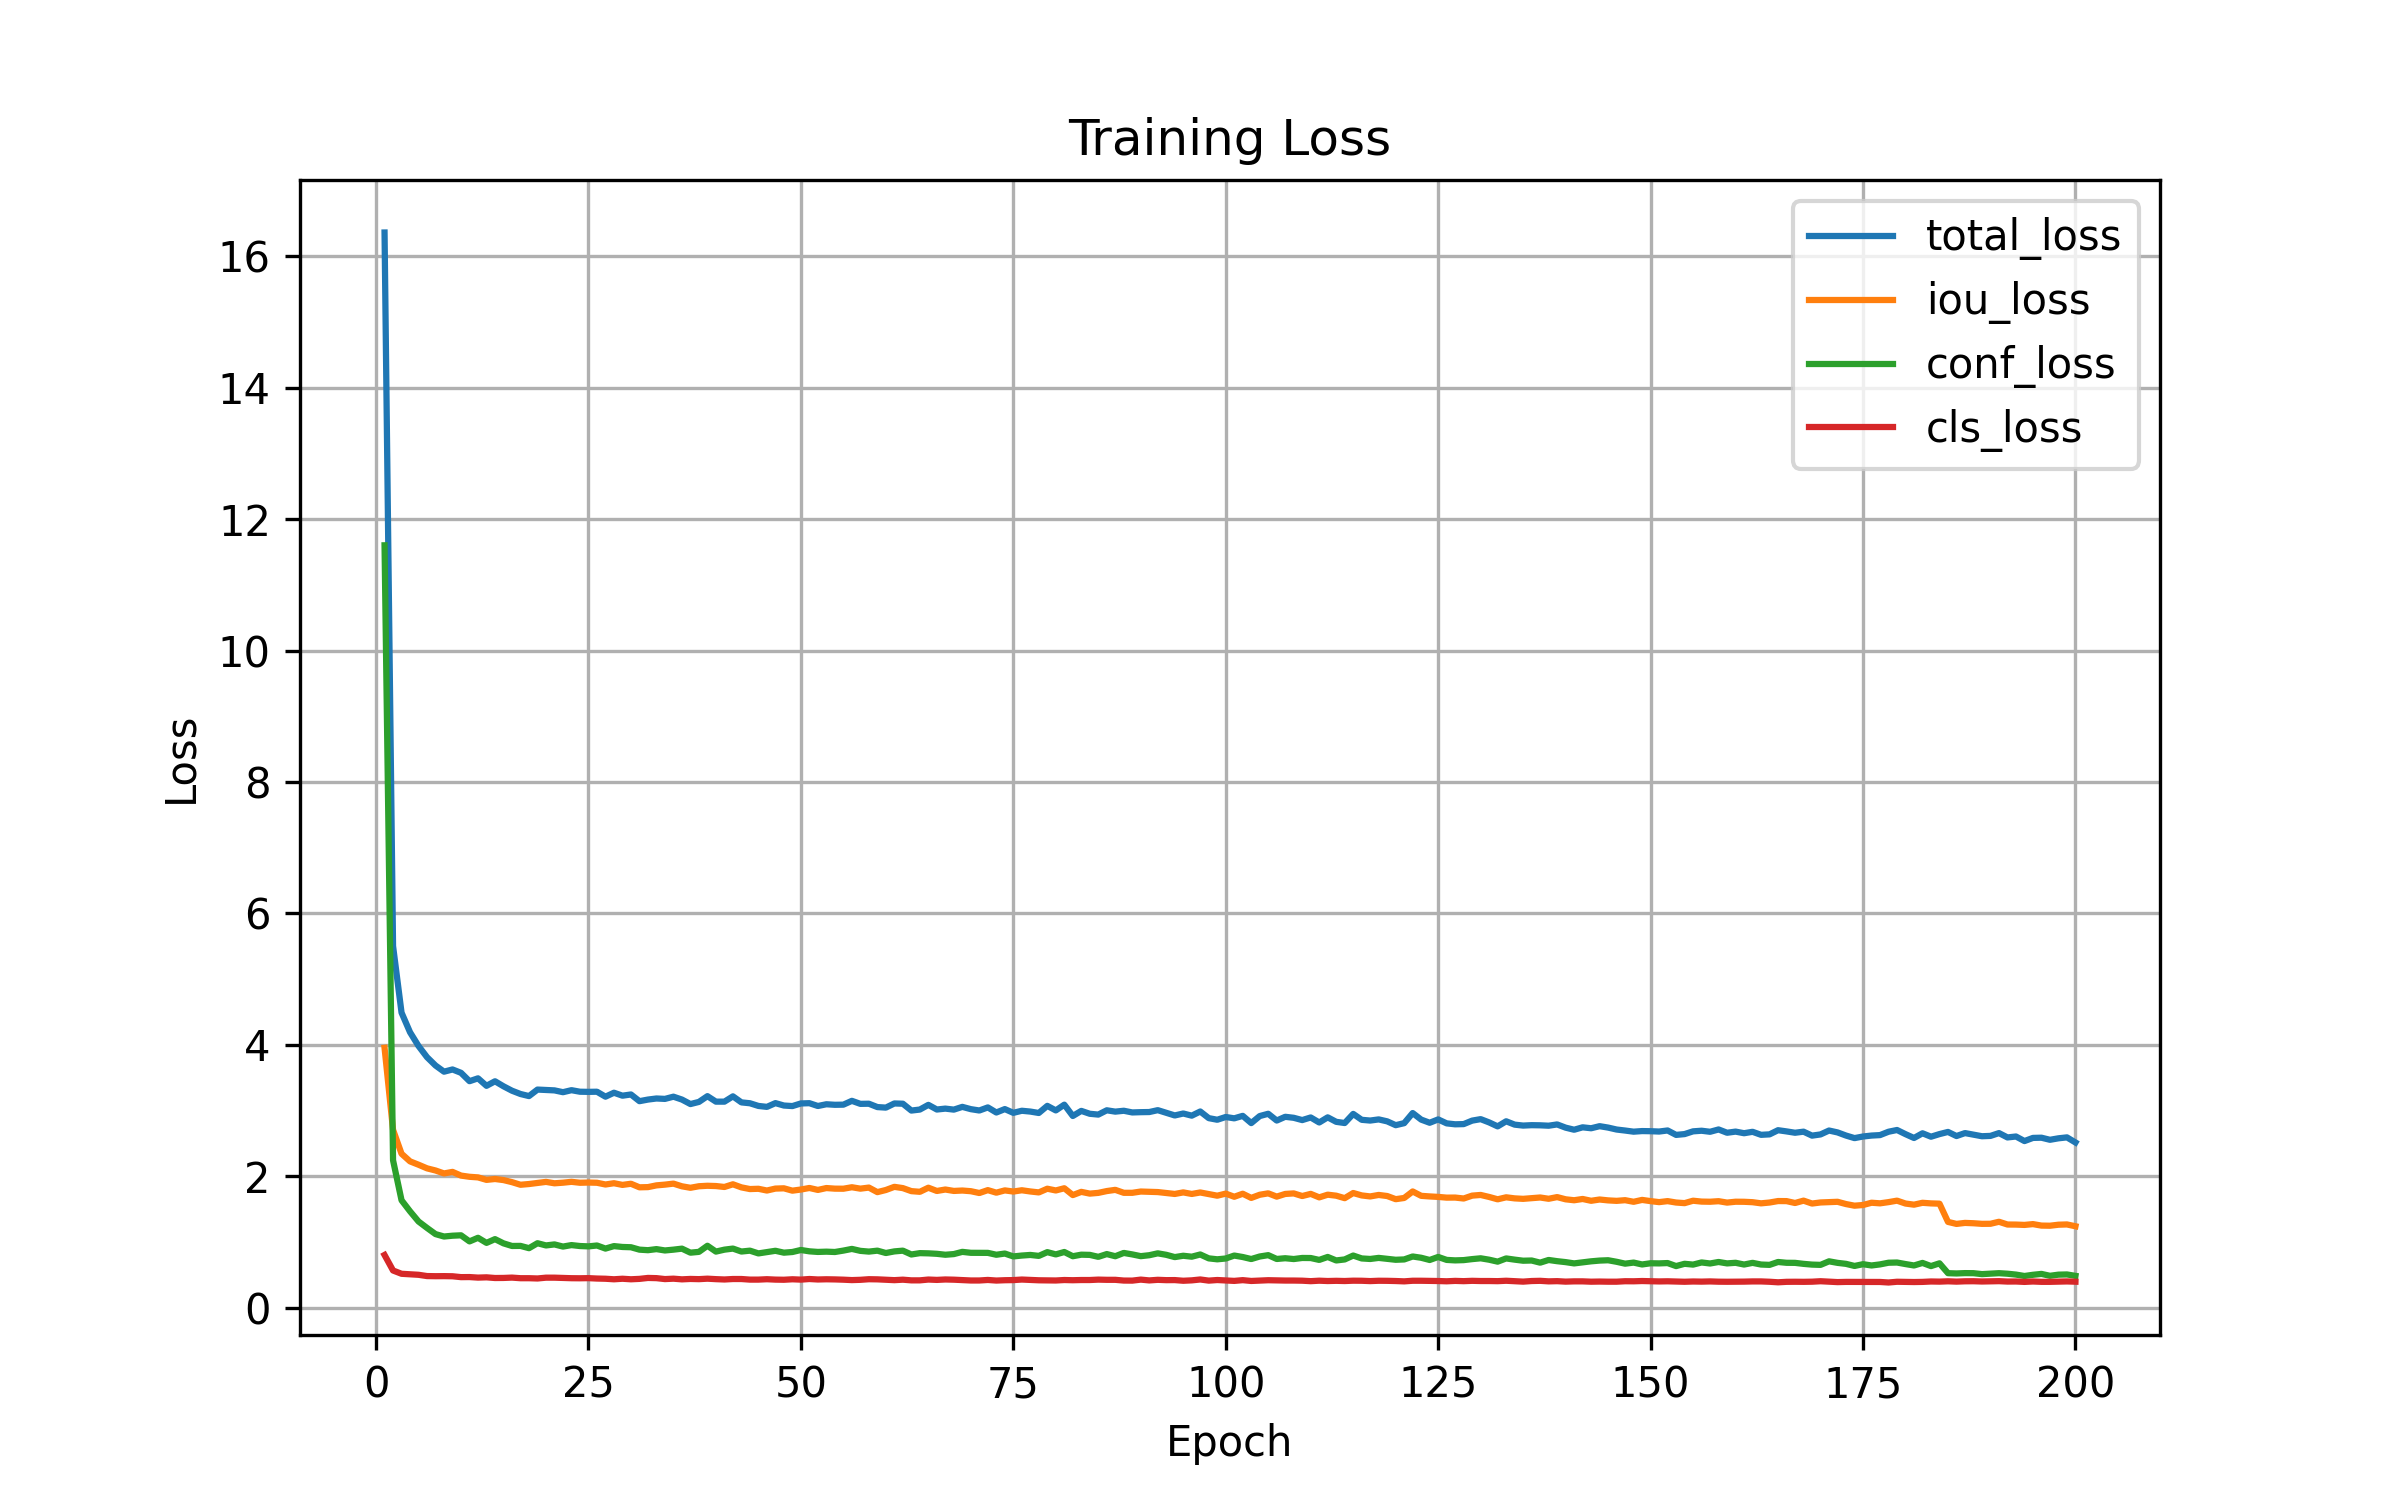
\includegraphics[width=\linewidth]{figures/images/chapter-11/licenseplate/v0/loss_curve.png}
\caption{Training loss}
\end{subfigure}
\hfill
\begin{subfigure}{0.48\textwidth}
\centering
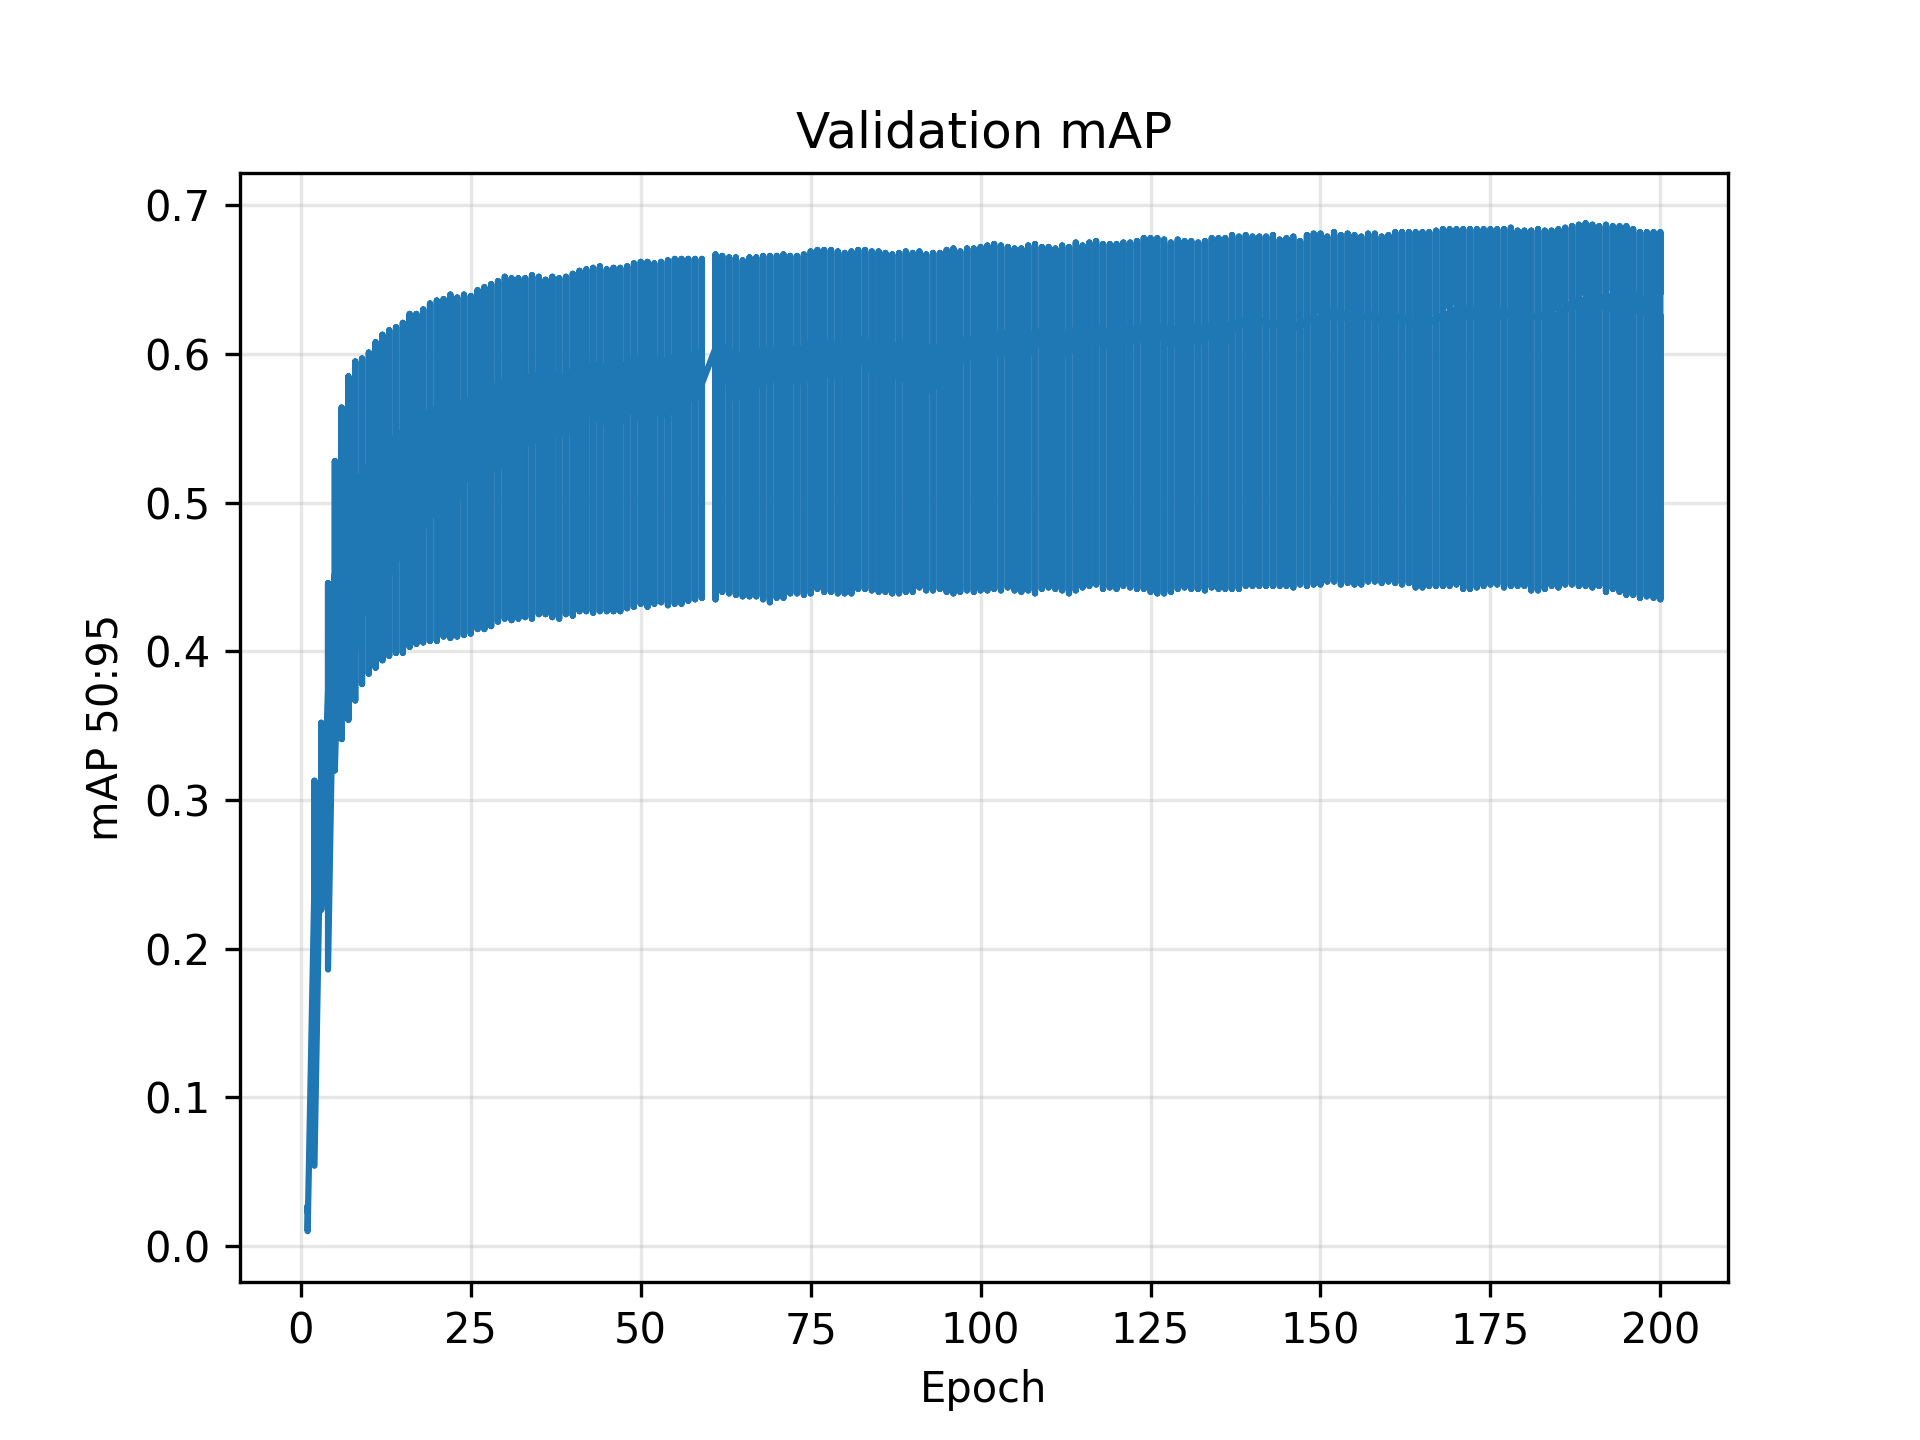
\includegraphics[width=\linewidth]{figures/images/chapter-11/licenseplate/v0/map_curve.png}
\caption{Validation mAP}
\end{subfigure}

\vspace{0.4cm}

\begin{subfigure}{0.50\textwidth}
\centering
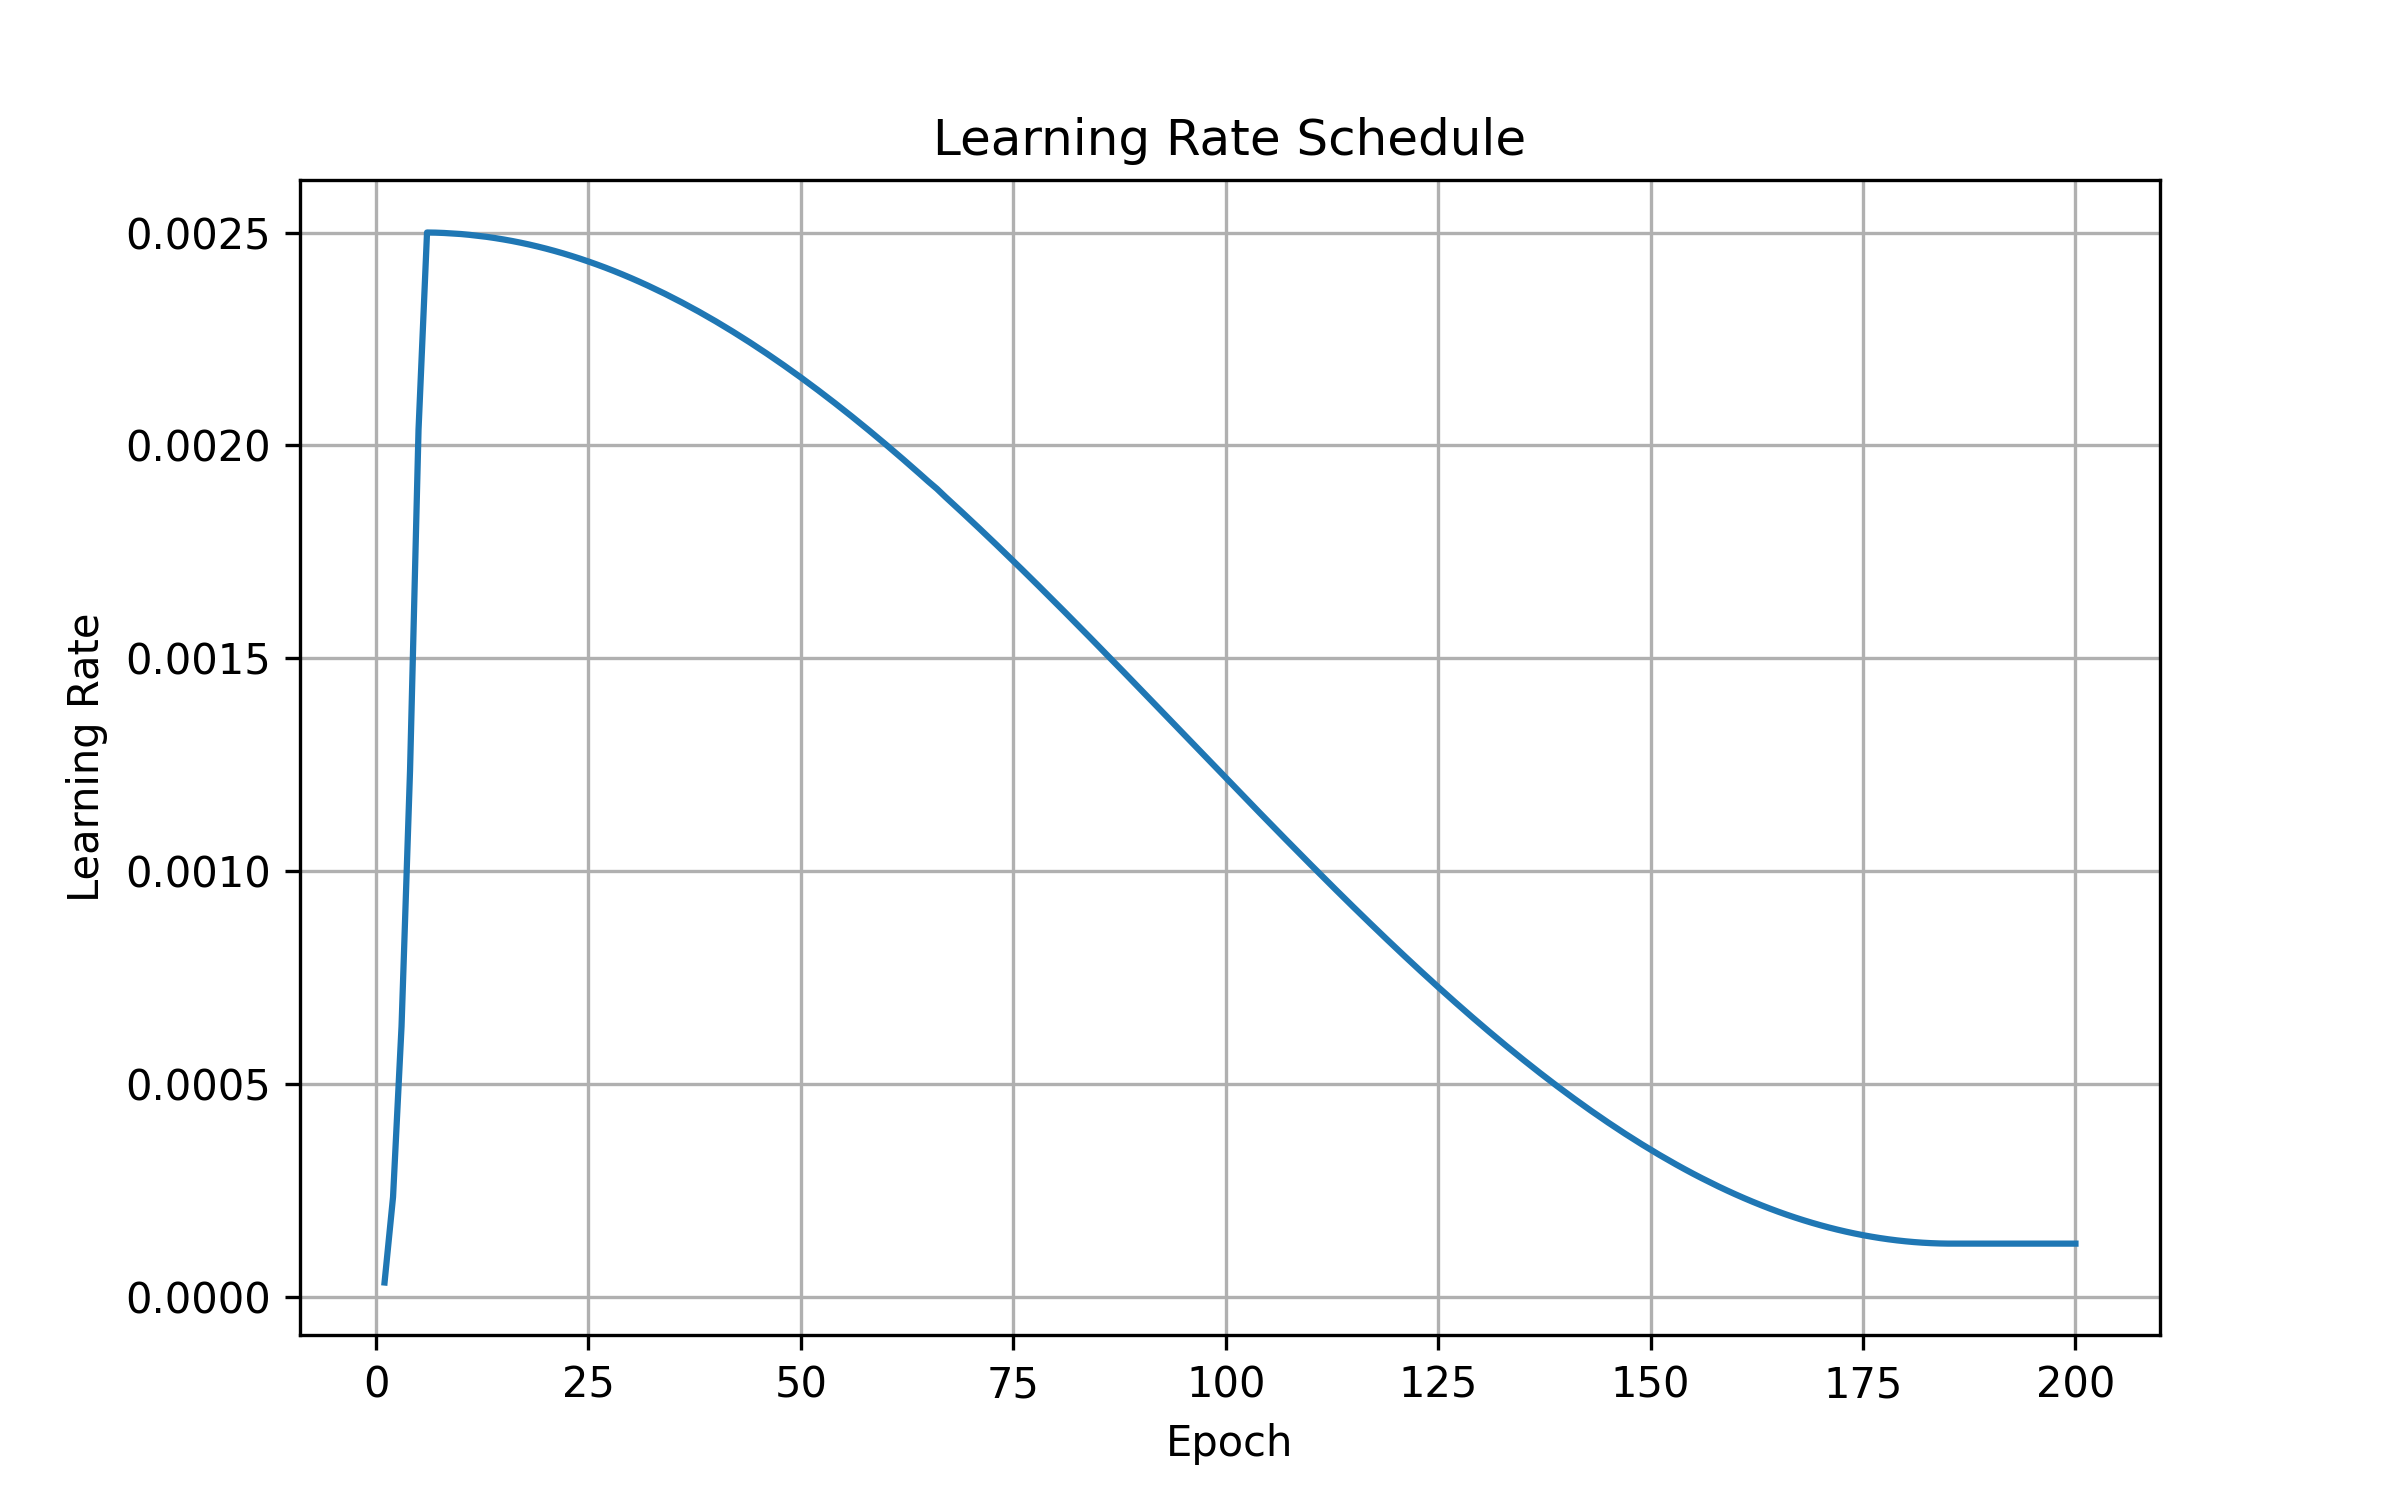
\includegraphics[width=\linewidth]{figures/images/chapter-11/licenseplate/v0/lr_curve.png}
\caption{Learning rate schedule}
\end{subfigure}

\caption{Training behavior of model v0.}
\label{fig:lp_training_v0}

\end{figure}

\begin{figure}[H]
\centering

\begin{subfigure}{0.50\textwidth}
\centering
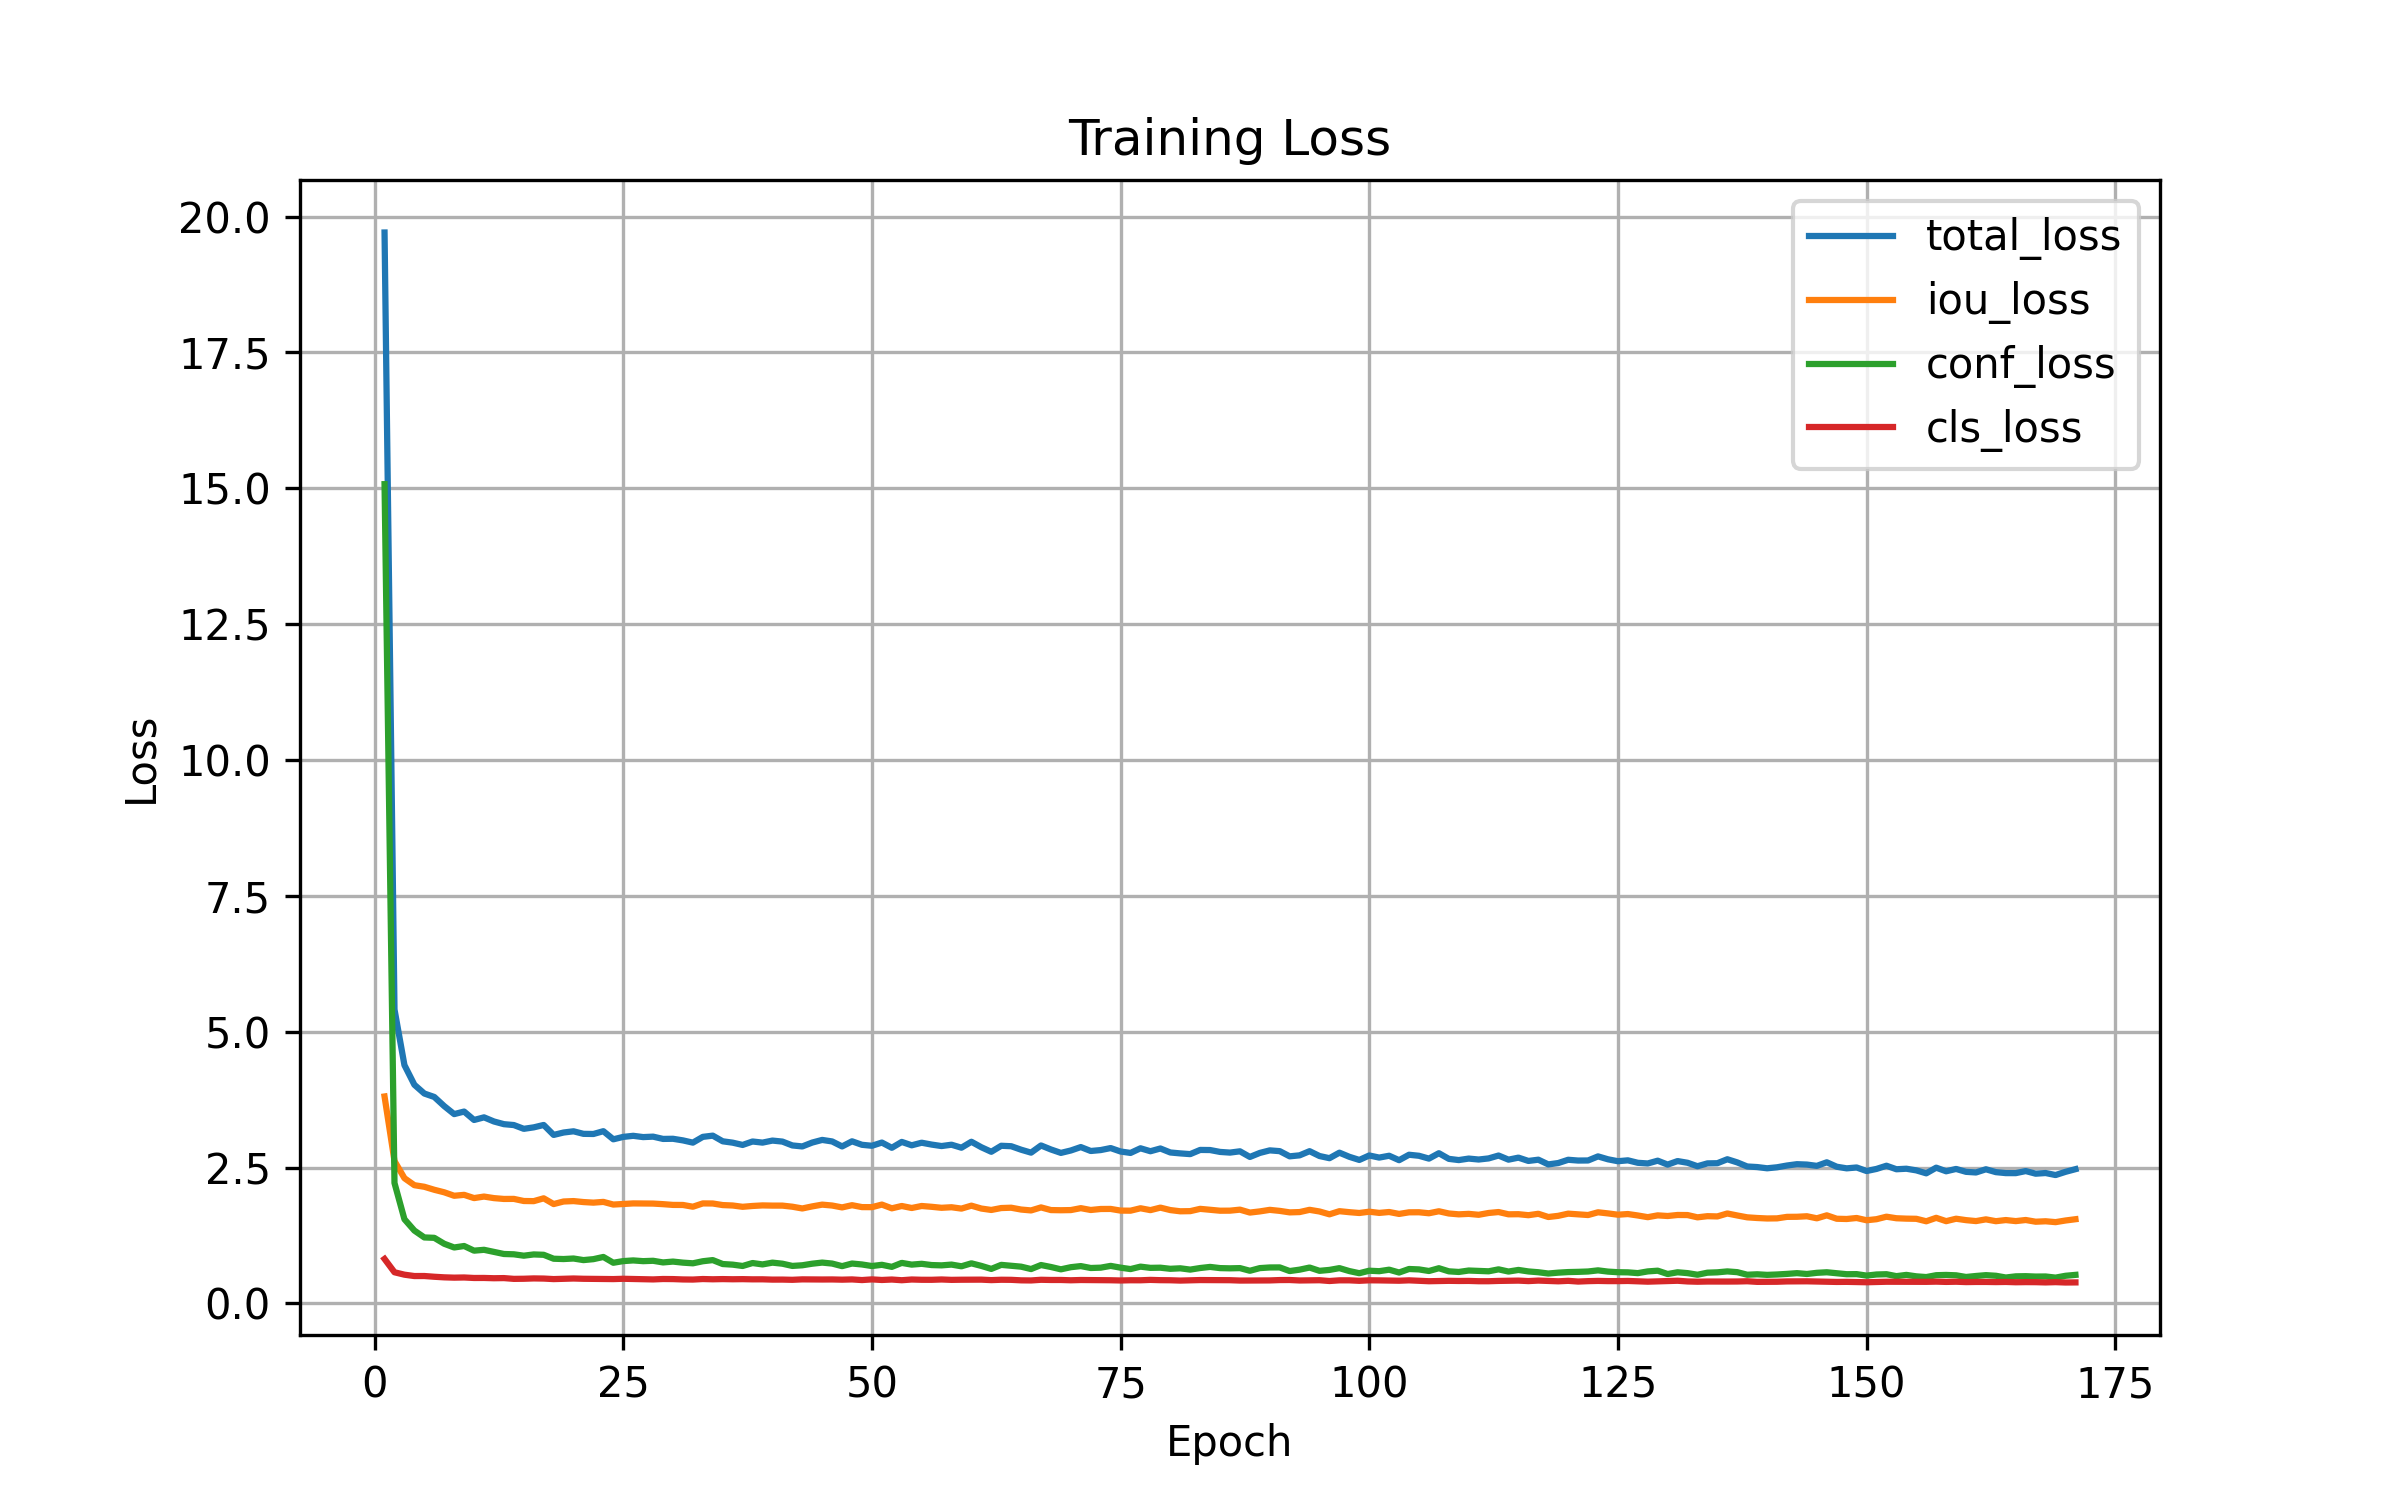
\includegraphics[width=\linewidth]{figures/images/chapter-11/licenseplate/v1/loss_curve.png}
\caption{Training loss}
\end{subfigure}
\hfill
\begin{subfigure}{0.48\textwidth}
\centering
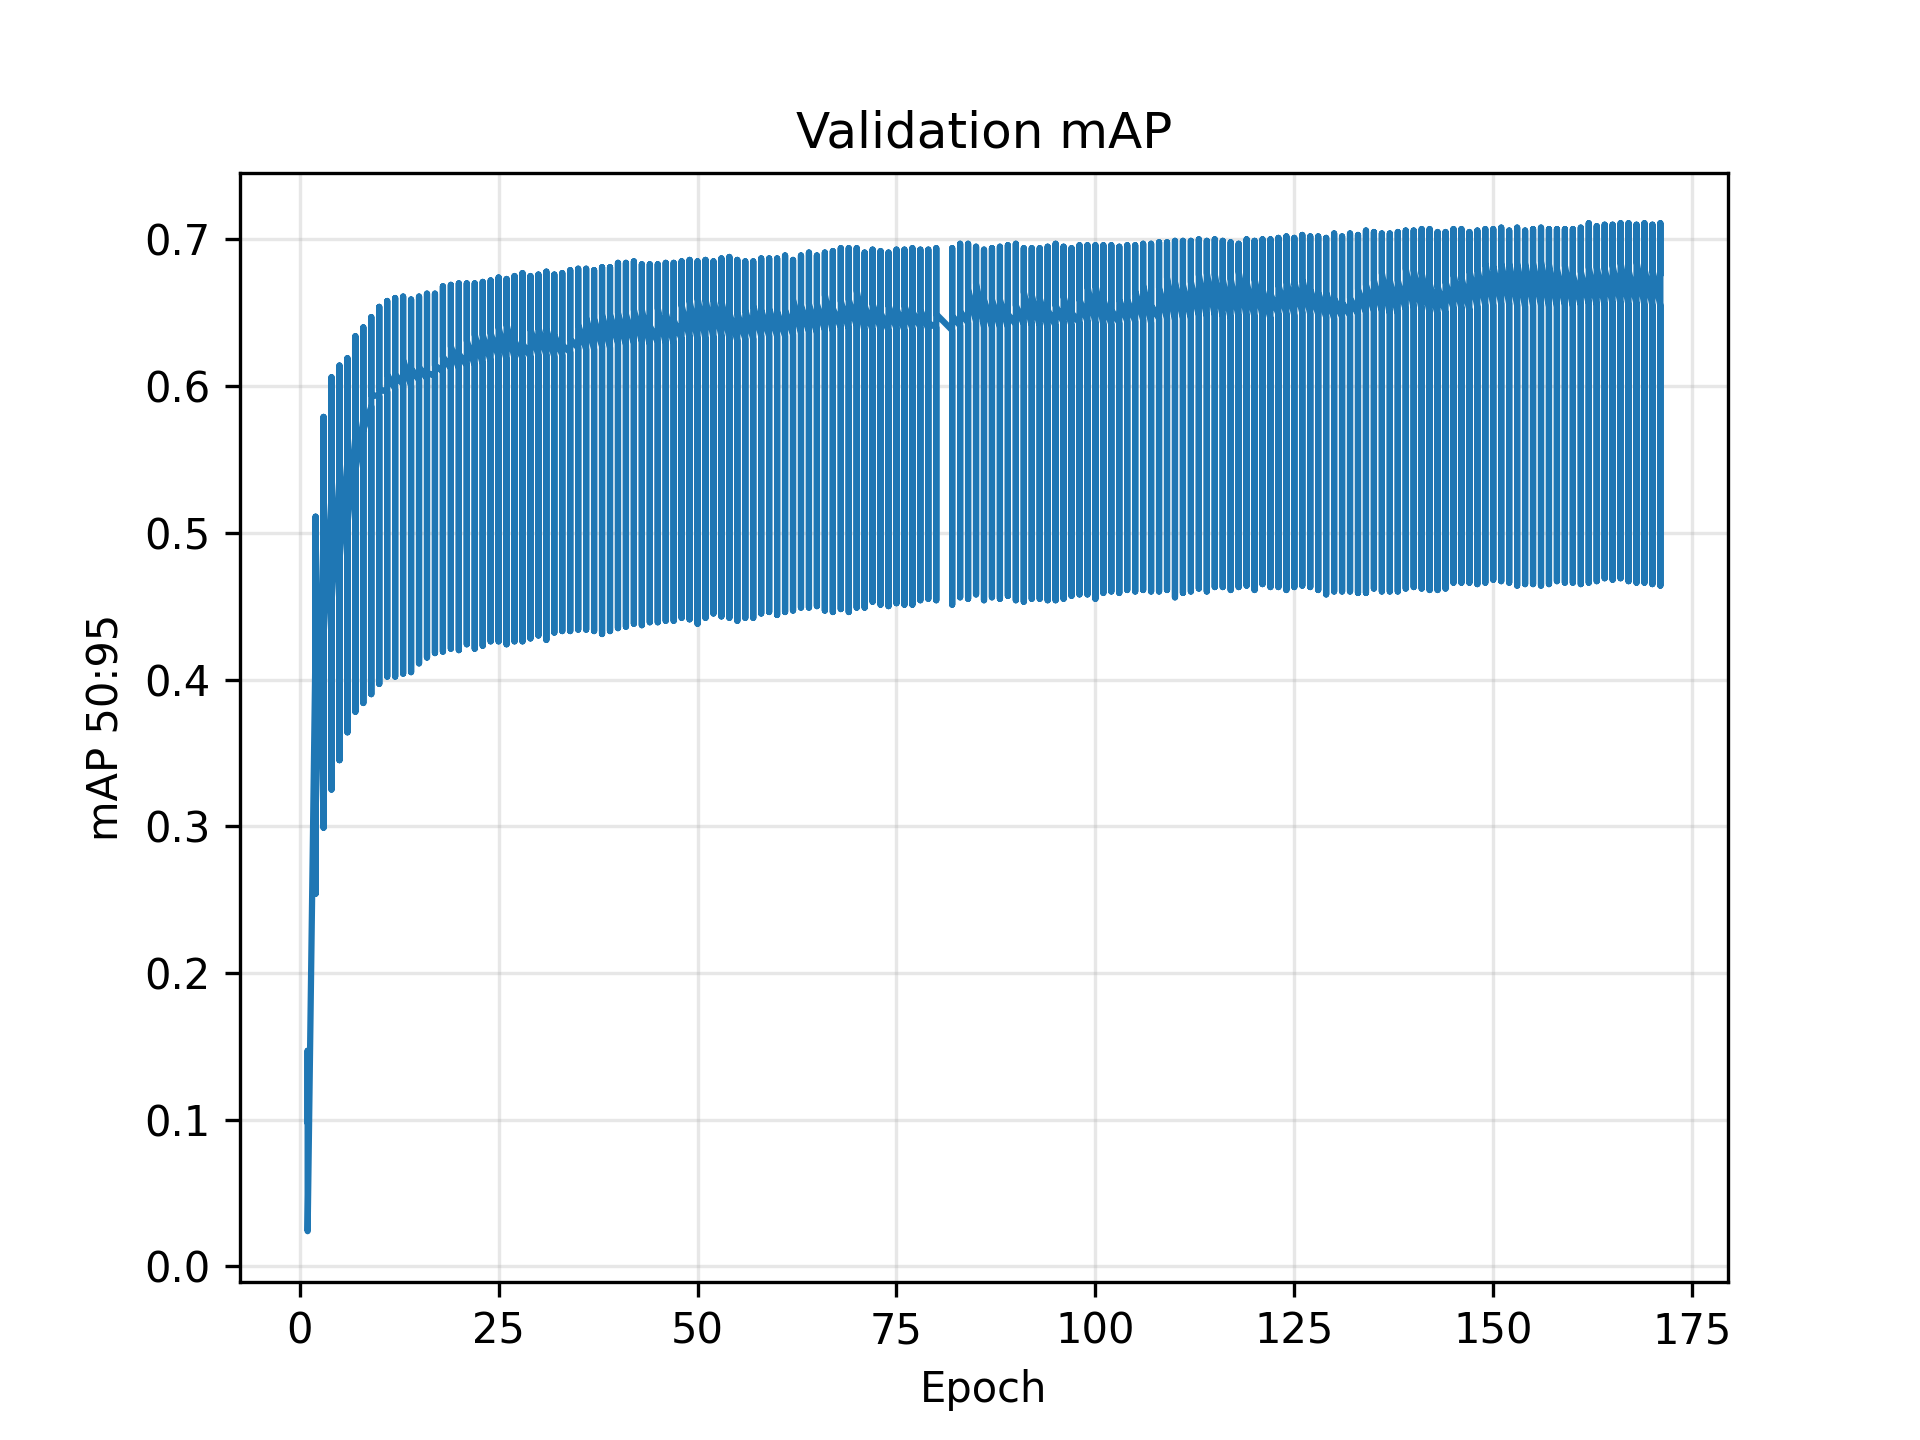
\includegraphics[width=\linewidth]{figures/images/chapter-11/licenseplate/v1/map_curve.png}
\caption{Validation mAP}
\end{subfigure}

\vspace{0.4cm}

\begin{subfigure}{0.50\textwidth}
\centering
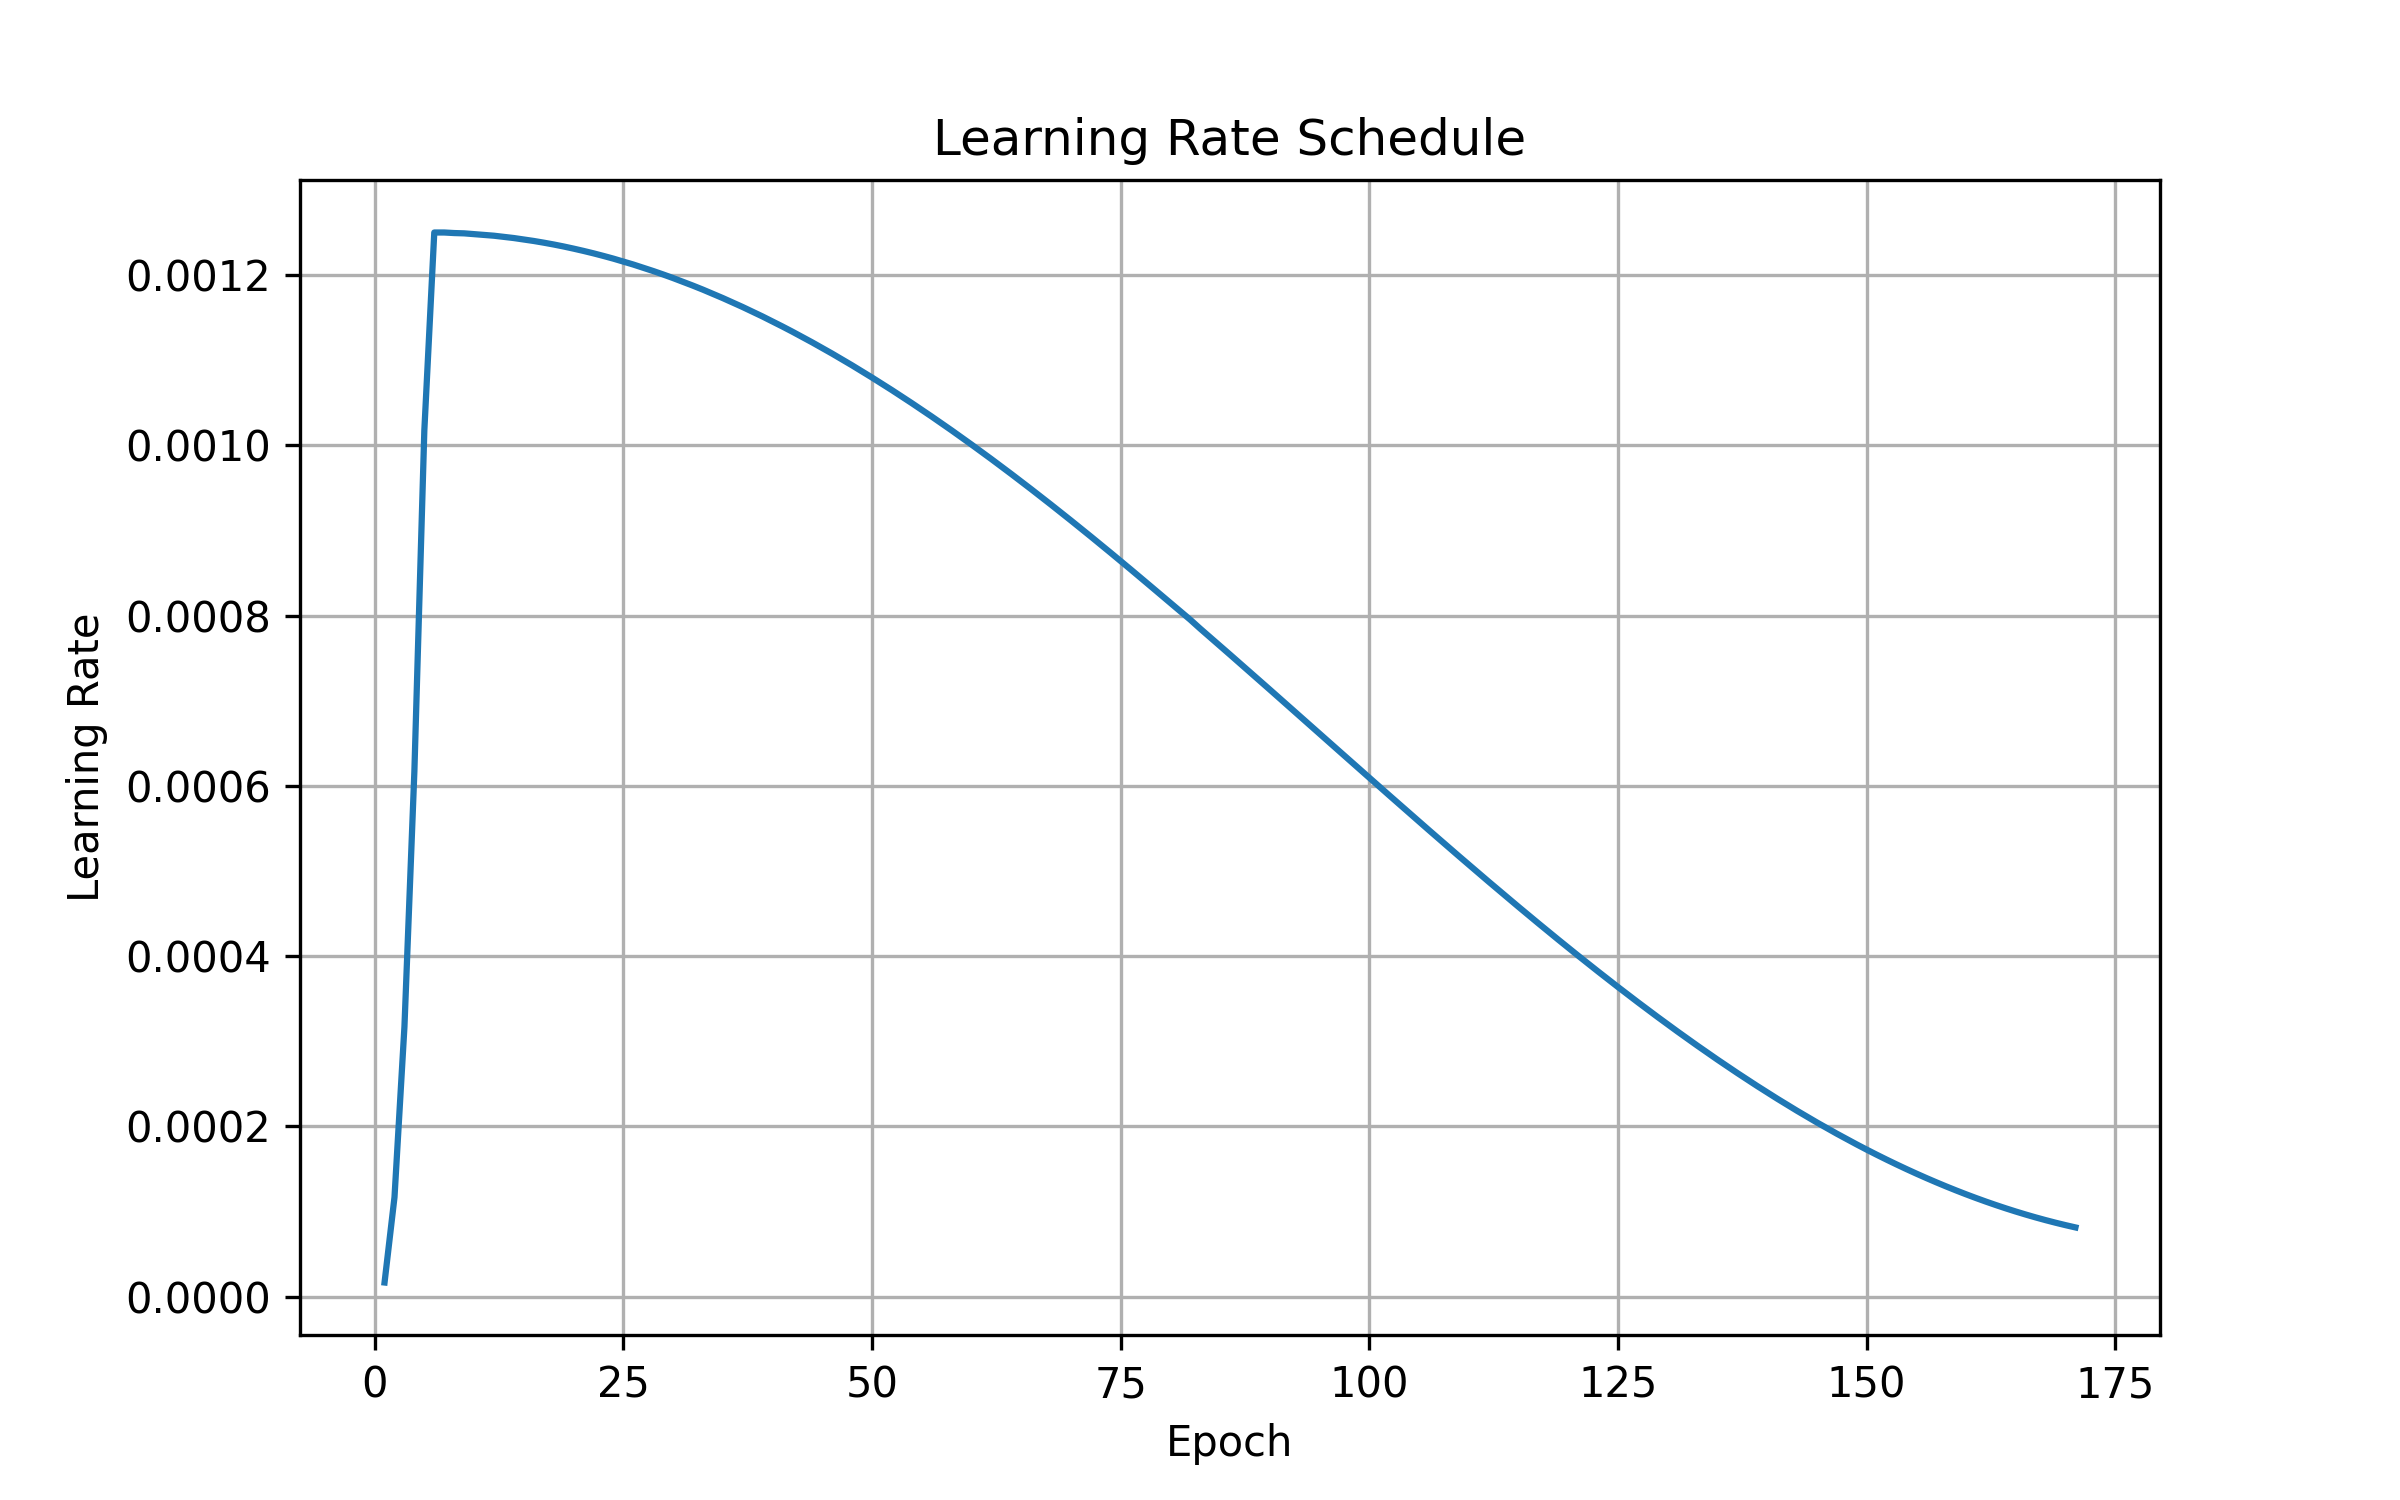
\includegraphics[width=\linewidth]{figures/images/chapter-11/licenseplate/v1/lr_curve.png}
\caption{Learning rate schedule}
\end{subfigure}

\caption{Training behavior of model v1.}
\label{fig:lp_training_v1}

\end{figure}

Figure~\ref{fig:lp_training_v0} and Figure~\ref{fig:lp_training_v1} show the
training behavior of the two license plate detection models. For both models,
the training loss decreases rapidly during the first epochs and then gradually
stabilizes, indicating stable optimization.

The validation mAP increases quickly at the beginning of training and then
continues to improve more gradually. Model v0 was trained for the full 200
epochs, while model v1 stopped earlier at approximately 175 epochs due to the
early stopping criterion. In both cases, the learning rate follows the expected
warm-up and decay schedule.







\subsection{Precision--Recall Analysis}

\begin{figure}[H]
\centering

\begin{subfigure}{0.48\textwidth}
\centering
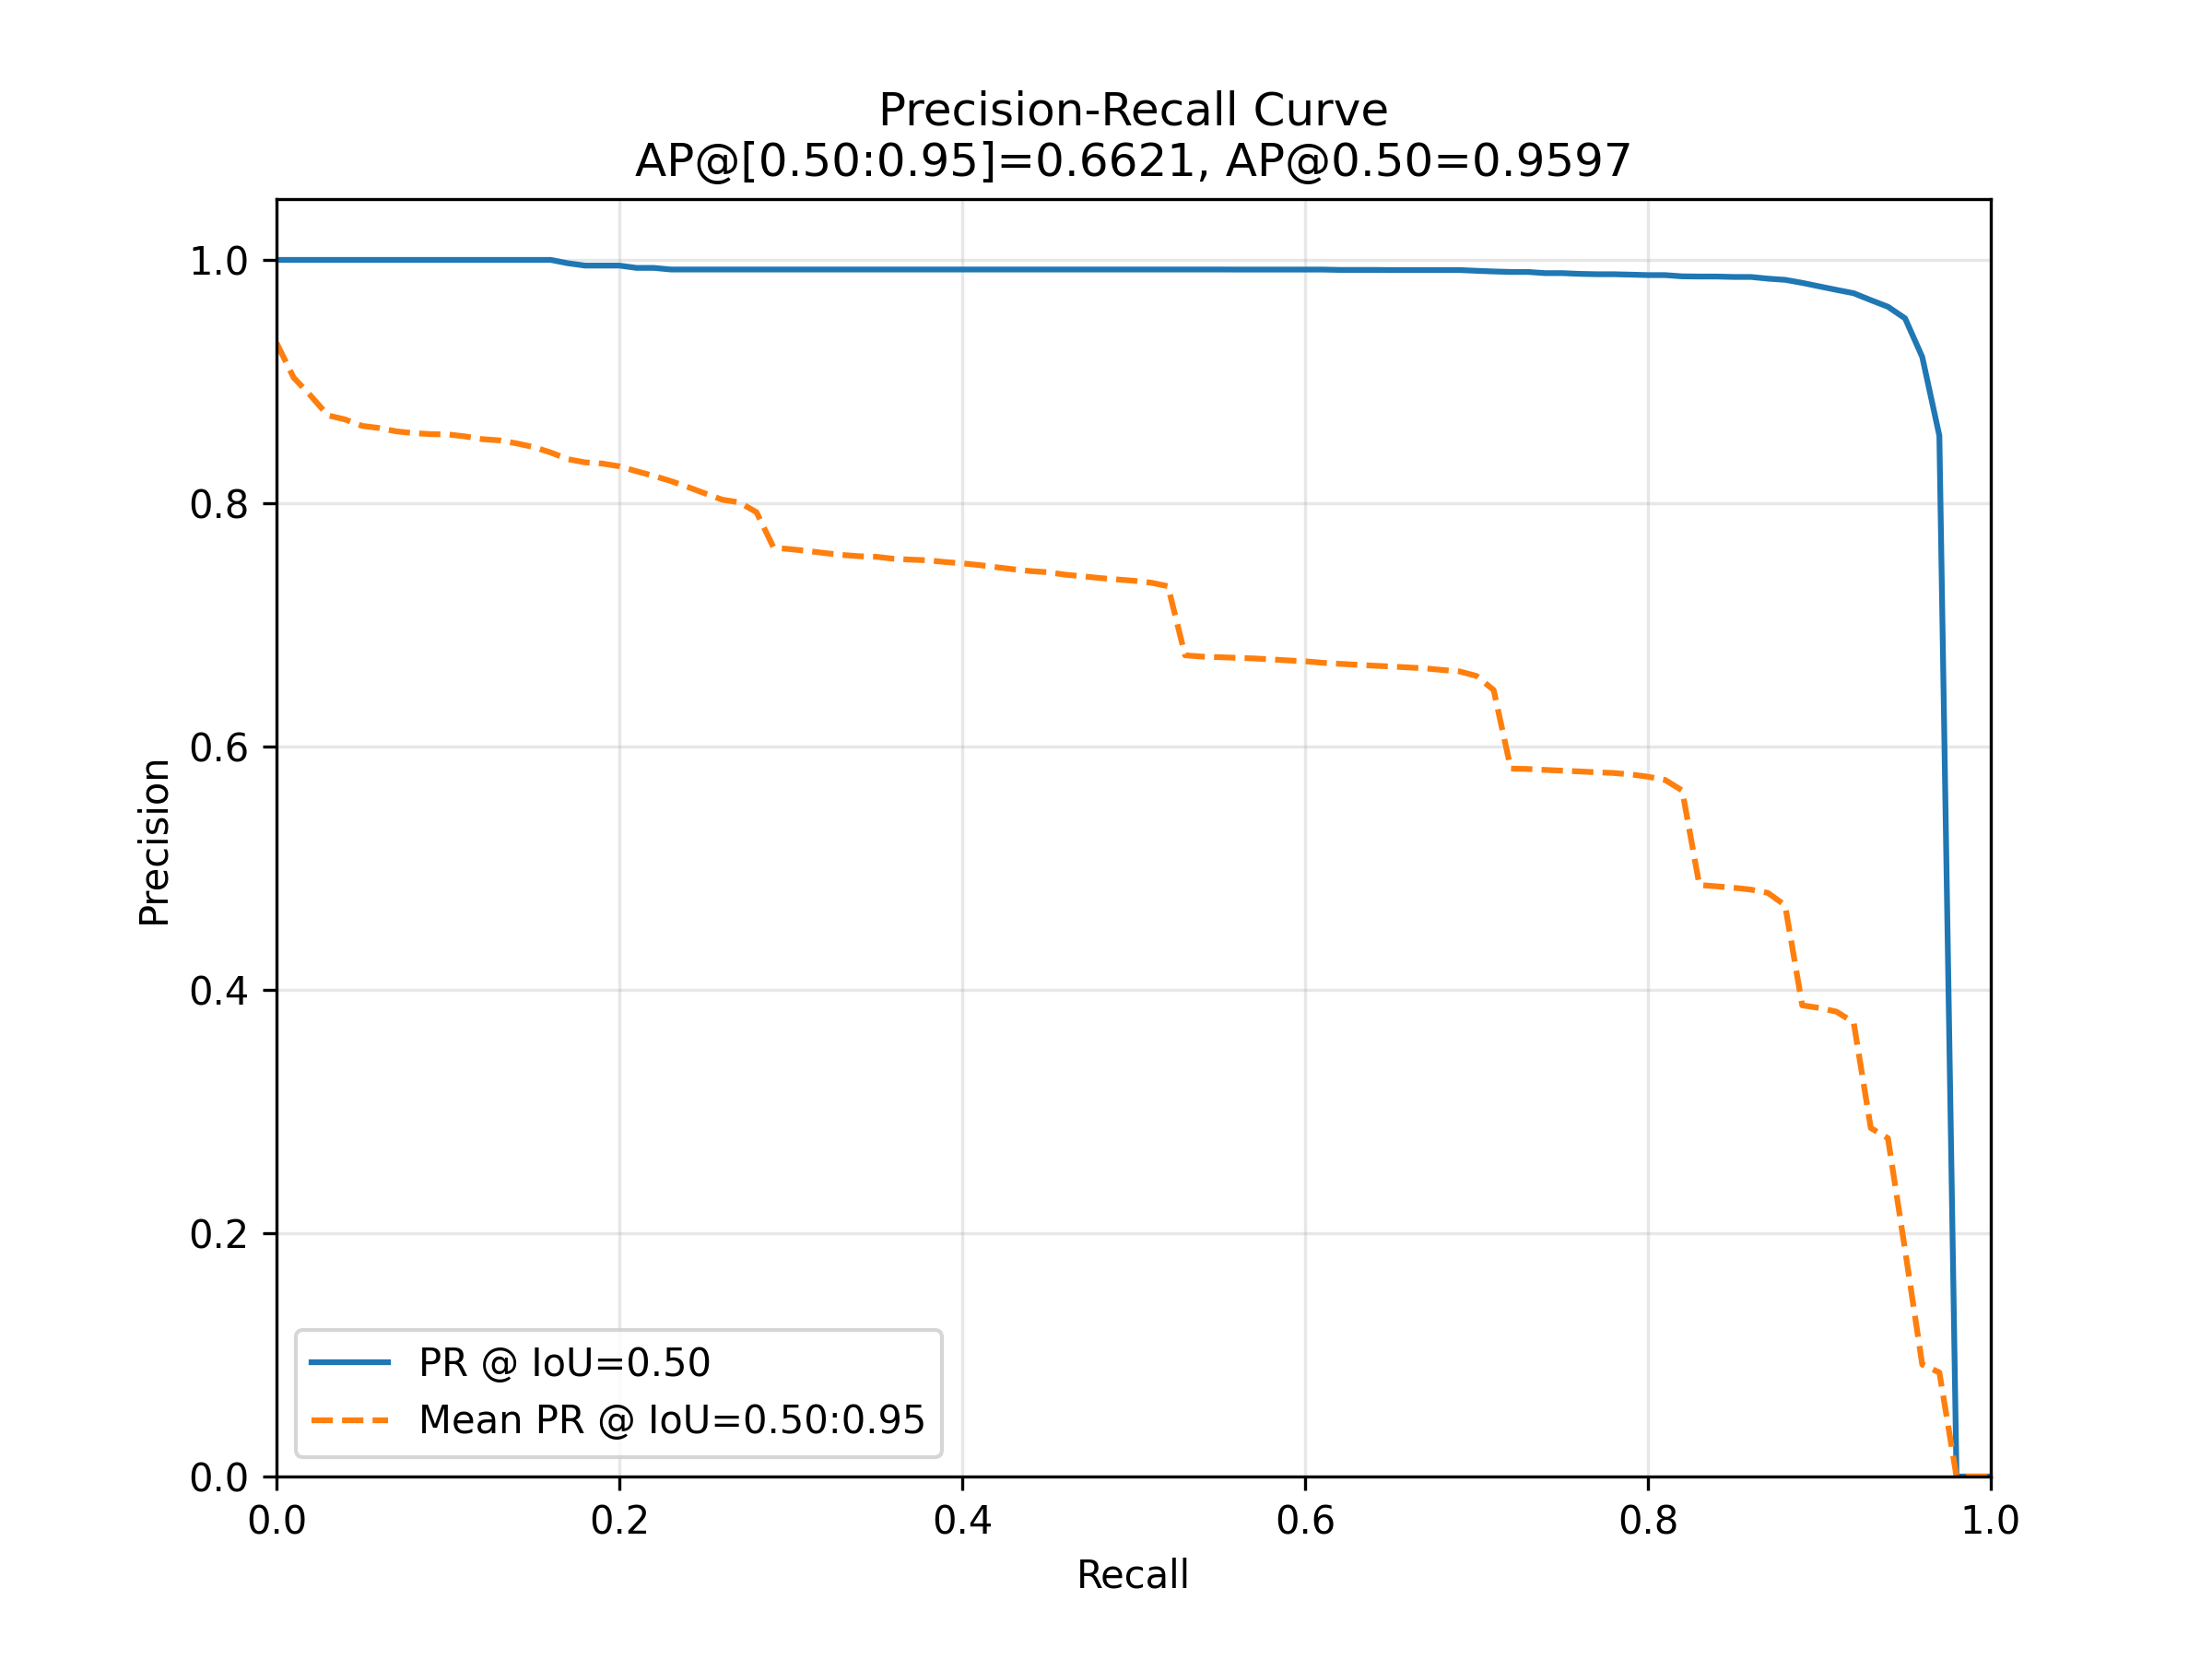
\includegraphics[width=\linewidth]{figures/images/chapter-11/licenseplate/v0/pr_curve.png}
\caption{V0 configuration.}
\end{subfigure}
\hfill
\begin{subfigure}{0.48\textwidth}
\centering
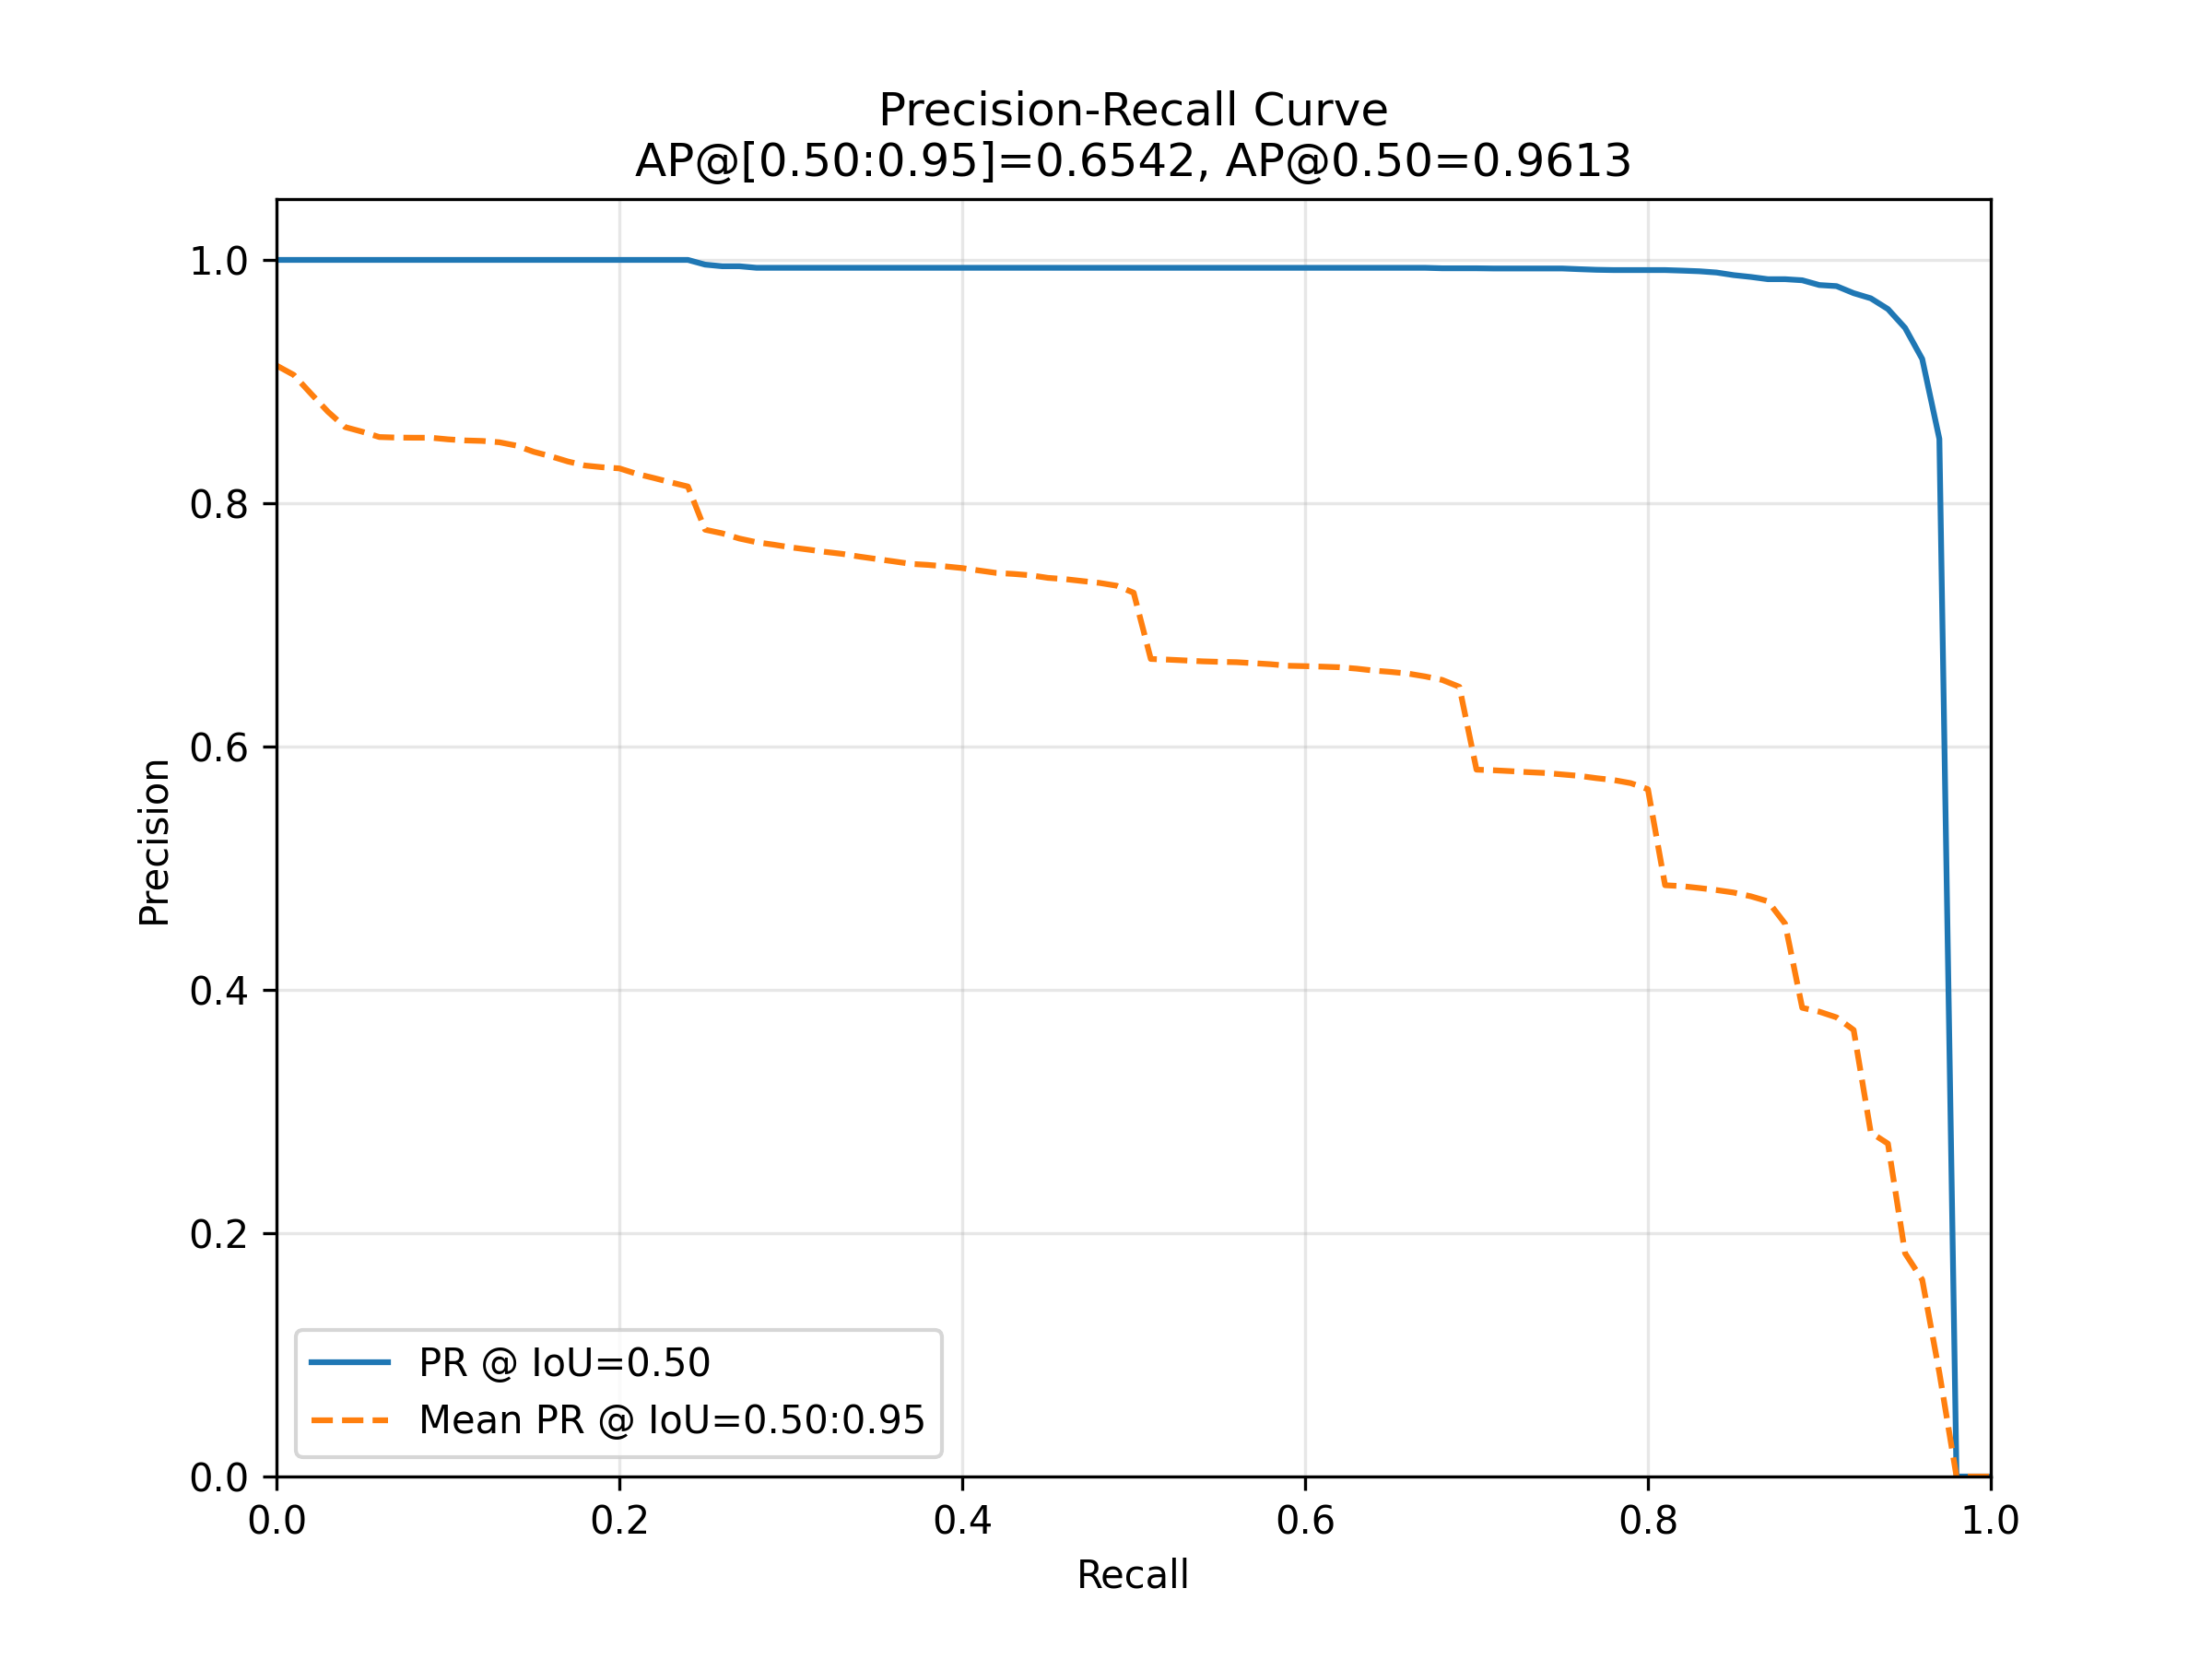
\includegraphics[width=\linewidth]{figures/images/chapter-11/licenseplate/v1/pr_curve.png}
\caption{V1 configuration.}
\end{subfigure}

\caption{Side-by-side comparison of the precision--recall curves for the v0 and v1 configurations.}
\label{fig:lp_pr_curves_licenseplate} 
\end{figure}

Figure~\ref{fig:lp_pr_curves_licenseplate} shows the precision--recall curves for the two
license plate detection models. Both configurations achieve a high AP@0.50,
with v0 reaching 0.9597 and v1 reaching 0.9613. This indicates strong detection
performance for both models at an IoU threshold of 0.50.

The AP@0.50:0.95 values are also similar, with v0 achieving 0.6621 and v1
achieving 0.6542. Although v1 performs slightly better at AP@0.50, v0 obtains a
slightly higher score across the stricter IoU range. Overall, the
precision--recall analysis shows that the two configurations perform similarly,
with only small differences between them.





\subsection{Confusion Matrix Analysis}

\begin{figure}[H]
\centering
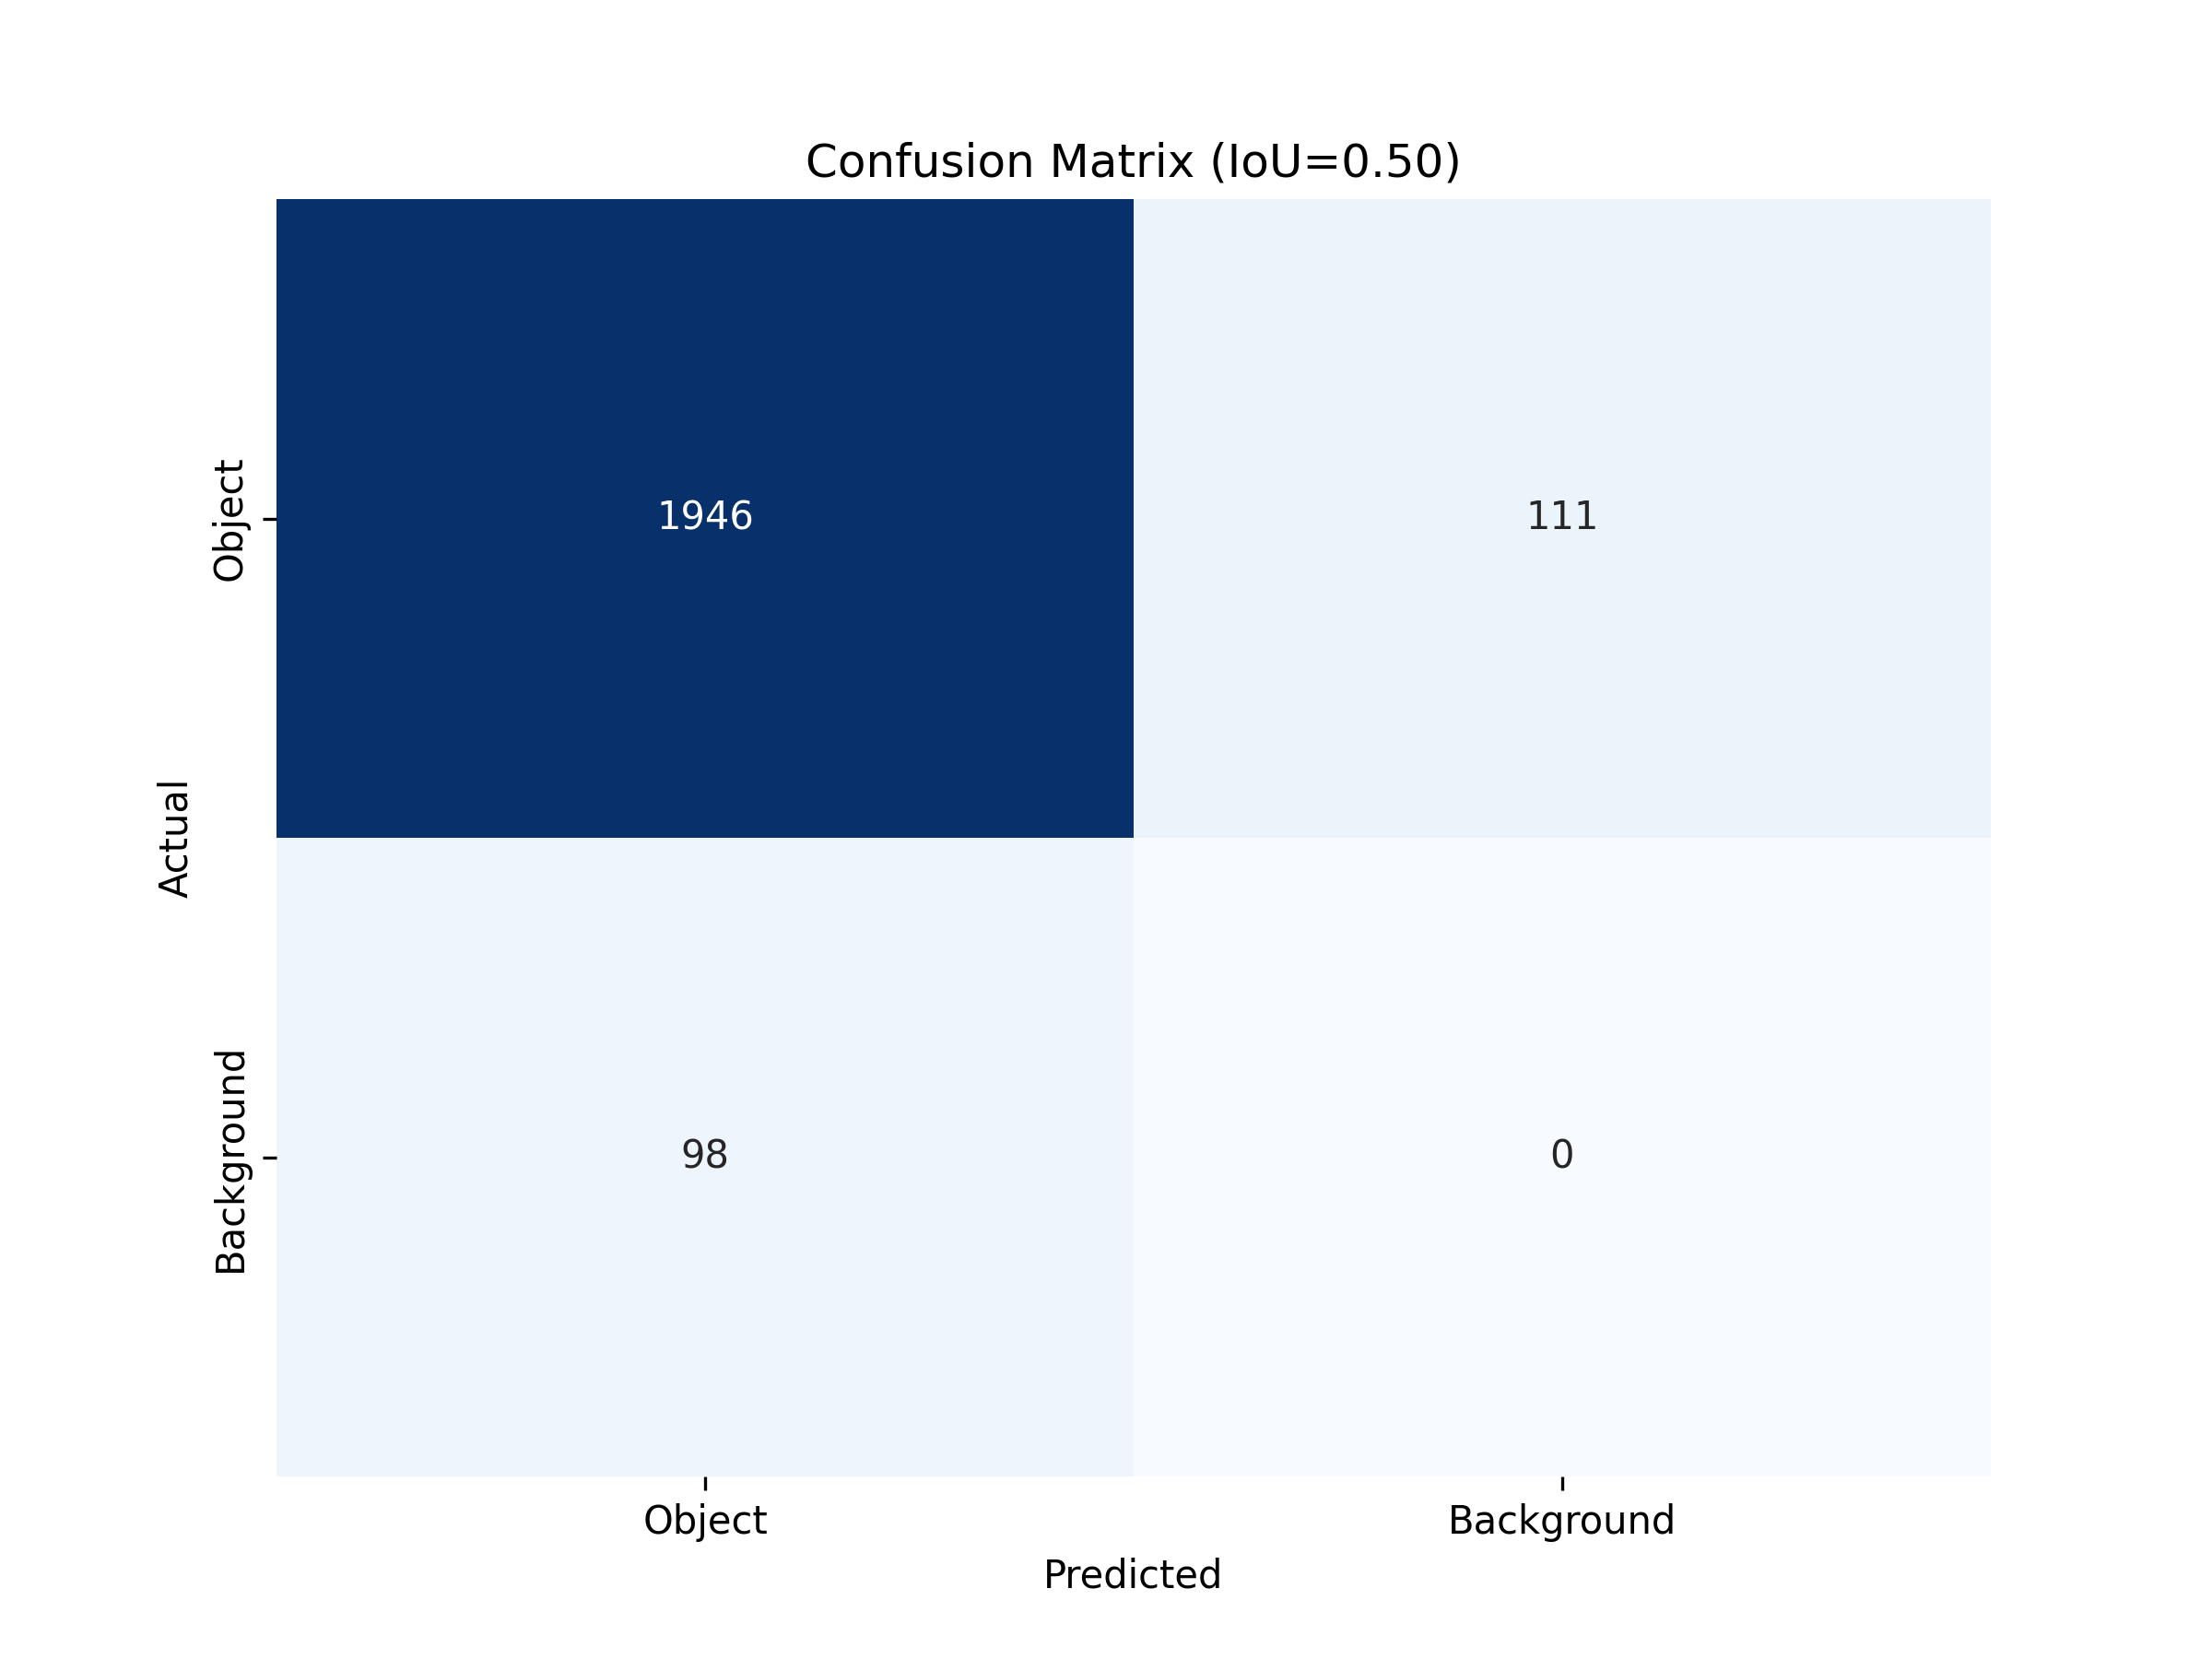
\includegraphics[width=12cm]{figures/images/chapter-11/licenseplate/v0/confusion_matrix_0.3.png}
\caption{Confusion matrix for the v0 configuration.}
\label{fig:lp_confusion_matrix_v0}
\end{figure}

\begin{figure}[H]
\centering
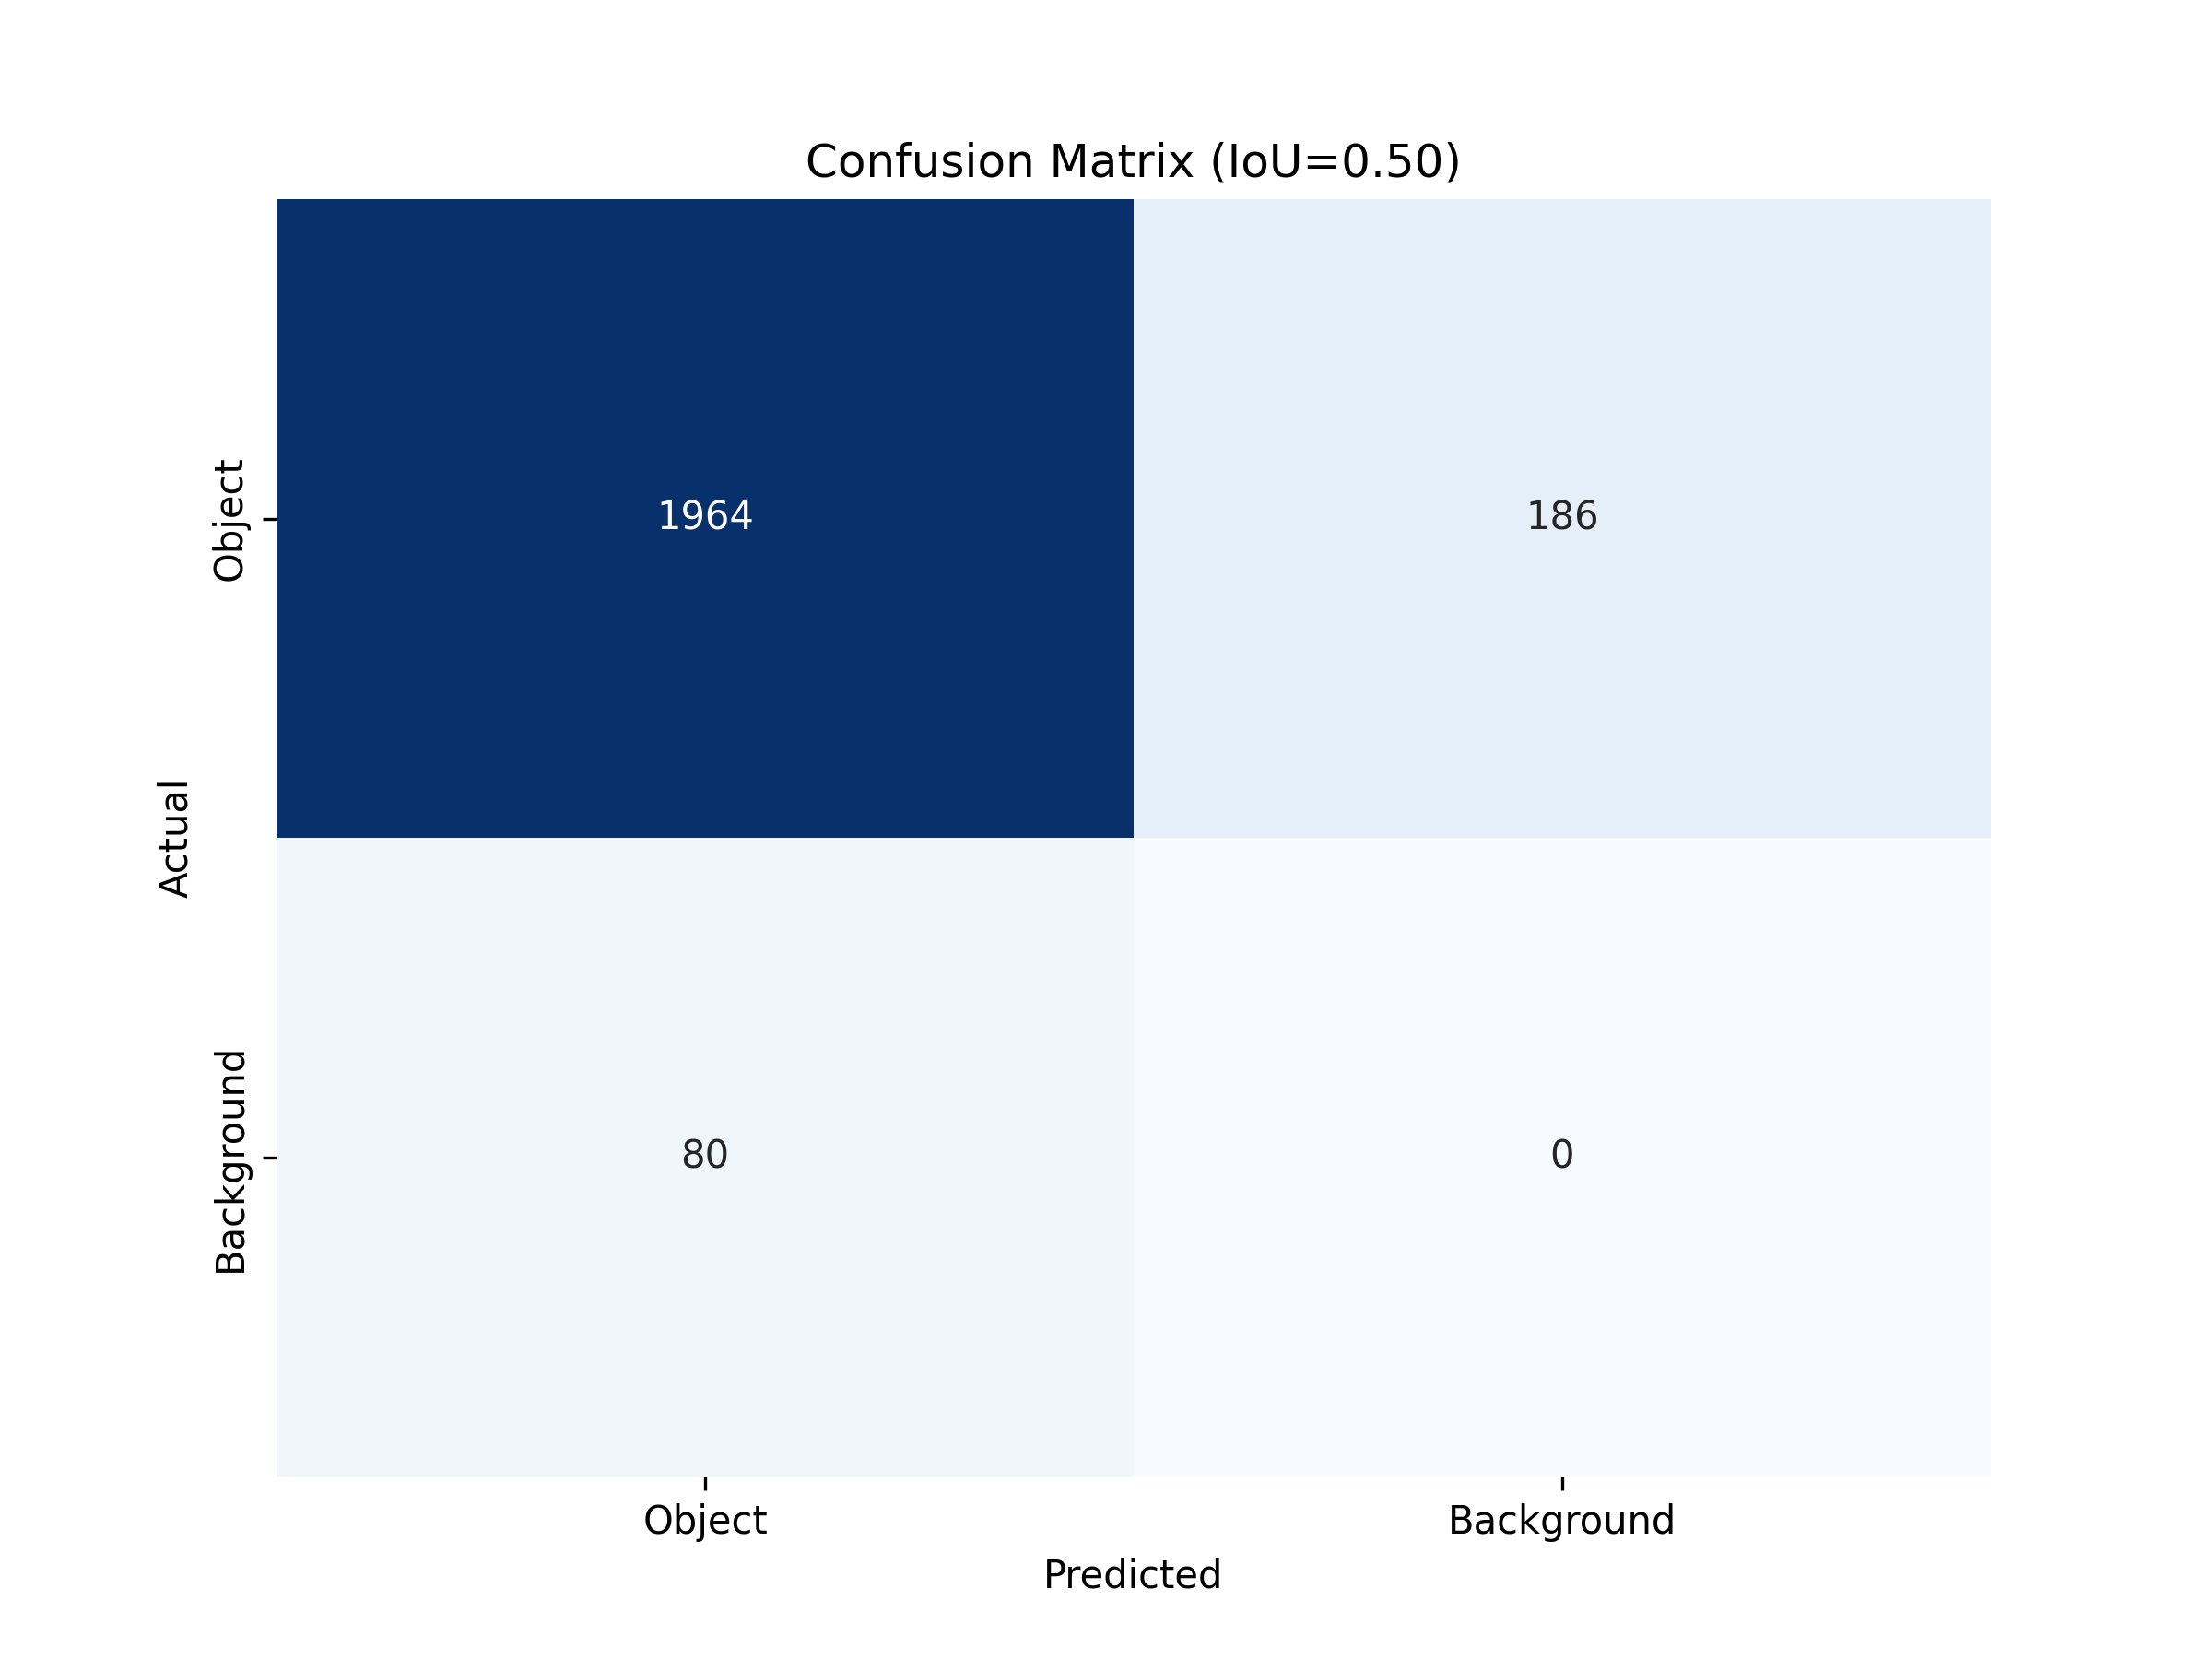
\includegraphics[width=12cm]{figures/images/chapter-11/licenseplate/v1/confusion_matrix_0.3.png}
\caption{Confusion matrix for the v1 configuration.}
\label{fig:lp_confusion_matrix_v1}
\end{figure}

Figure~\ref{fig:lp_confusion_matrix_v0} and
Figure~\ref{fig:lp_confusion_matrix_v1} show the confusion matrices for the two
license plate detection models at an IoU threshold of 0.50.

The confusion matrix values do not directly match the number of test images
because object detection is evaluated at the object level. Each image may
contain multiple license plates and multiple predicted bounding boxes.
Therefore, the matrix counts detections and missed objects rather than images.

The F1-score was calculated as the harmonic mean of precision and recall:
\[
F1 = 2 \cdot \frac{Precision \cdot Recall}{Precision + Recall}
\]

The v0 configuration correctly detected 1946 license plates, produced 98 false
positive detections, and missed 111 license plates. This resulted in a
precision of 0.9521, a recall of 0.9460, and an F1-score of 0.9490.

The v1 configuration correctly detected 1964 license plates and produced fewer
false positives, with 80 false detections. However, it also missed more license
plates, with 186 false negatives. This resulted in a slightly higher precision
of 0.9609, but a lower recall of 0.9135 and an F1-score of 0.9366.

\begin{align*}
Precision_{v0} &= \frac{1946}{1946 + 98} \approx 0.9521,
&
Recall_{v0} &= \frac{1946}{1946 + 111} \approx 0.9460,
&
F1_{v0} &\approx 0.9490
\end{align*}

\begin{align*}
Precision_{v1} &= \frac{1964}{1964 + 80} \approx 0.9609,
&
Recall_{v1} &= \frac{1964}{1964 + 186} \approx 0.9135,
&
F1_{v1} &\approx 0.9366
\end{align*}

Overall, v1 is slightly more precise, while v0 achieves better recall and a
higher F1-score. This indicates that v0 provides a better balance between
detecting license plates and avoiding false detections.

\subsection{Summary}